\begin{anexosenv}

\partanexos

\chapter{Integração Contínua}
\begin{python}[caption={Exemplo de integração contínua do SMI-UnB}, captionpos=b, label={integracao_cont}]
Running with gitlab-ci-multi-runner 9.3.0-rc.2 (110d530)
  on docker-auto-scale (e11ae361)
Using Docker executor with image python:3.5 ...
Starting service postgres:latest ...
Pulling docker image postgres:latest ...
Using docker image postgres:latest for postgres service...
Waiting for services to be up and running...
Using docker image sha256 for predefined container...
Pulling docker image python:3.5 ...
Using docker image python:3.5 for build container...
Running on runner-e11ae361-project-1216906...
Cloning repository...
Cloning into '/builds/brenddongontijo/SMI-UnB'...
Checking out e70a256f as master...
Skipping Git submodules setup
$ apt-get update -qq
$ apt-get install python3-pip -y -qq
# Installing packages...
$ flake8 src/ --exclude migrations
$ coverage run manage.py test \
smi_unb --settings=smi_unb.settings_runner
# Running tests...
----------------------------------------------
Ran 192 tests in 17.081s
OK
Creating a new SECRET_KEY at security/secret_key.dat
Running server in DEBUG mode. Plese do *not* go to production!
Documentation files not found: disabling tests!
Creating test database for alias 'default'...
Destroying test database for alias 'default'...
$ coverage report
# Coverage report...
Job succeeded
\end{python}

\chapter{Cobertura Total de Código}
\begin{figure}[!htpb]
    \centering
    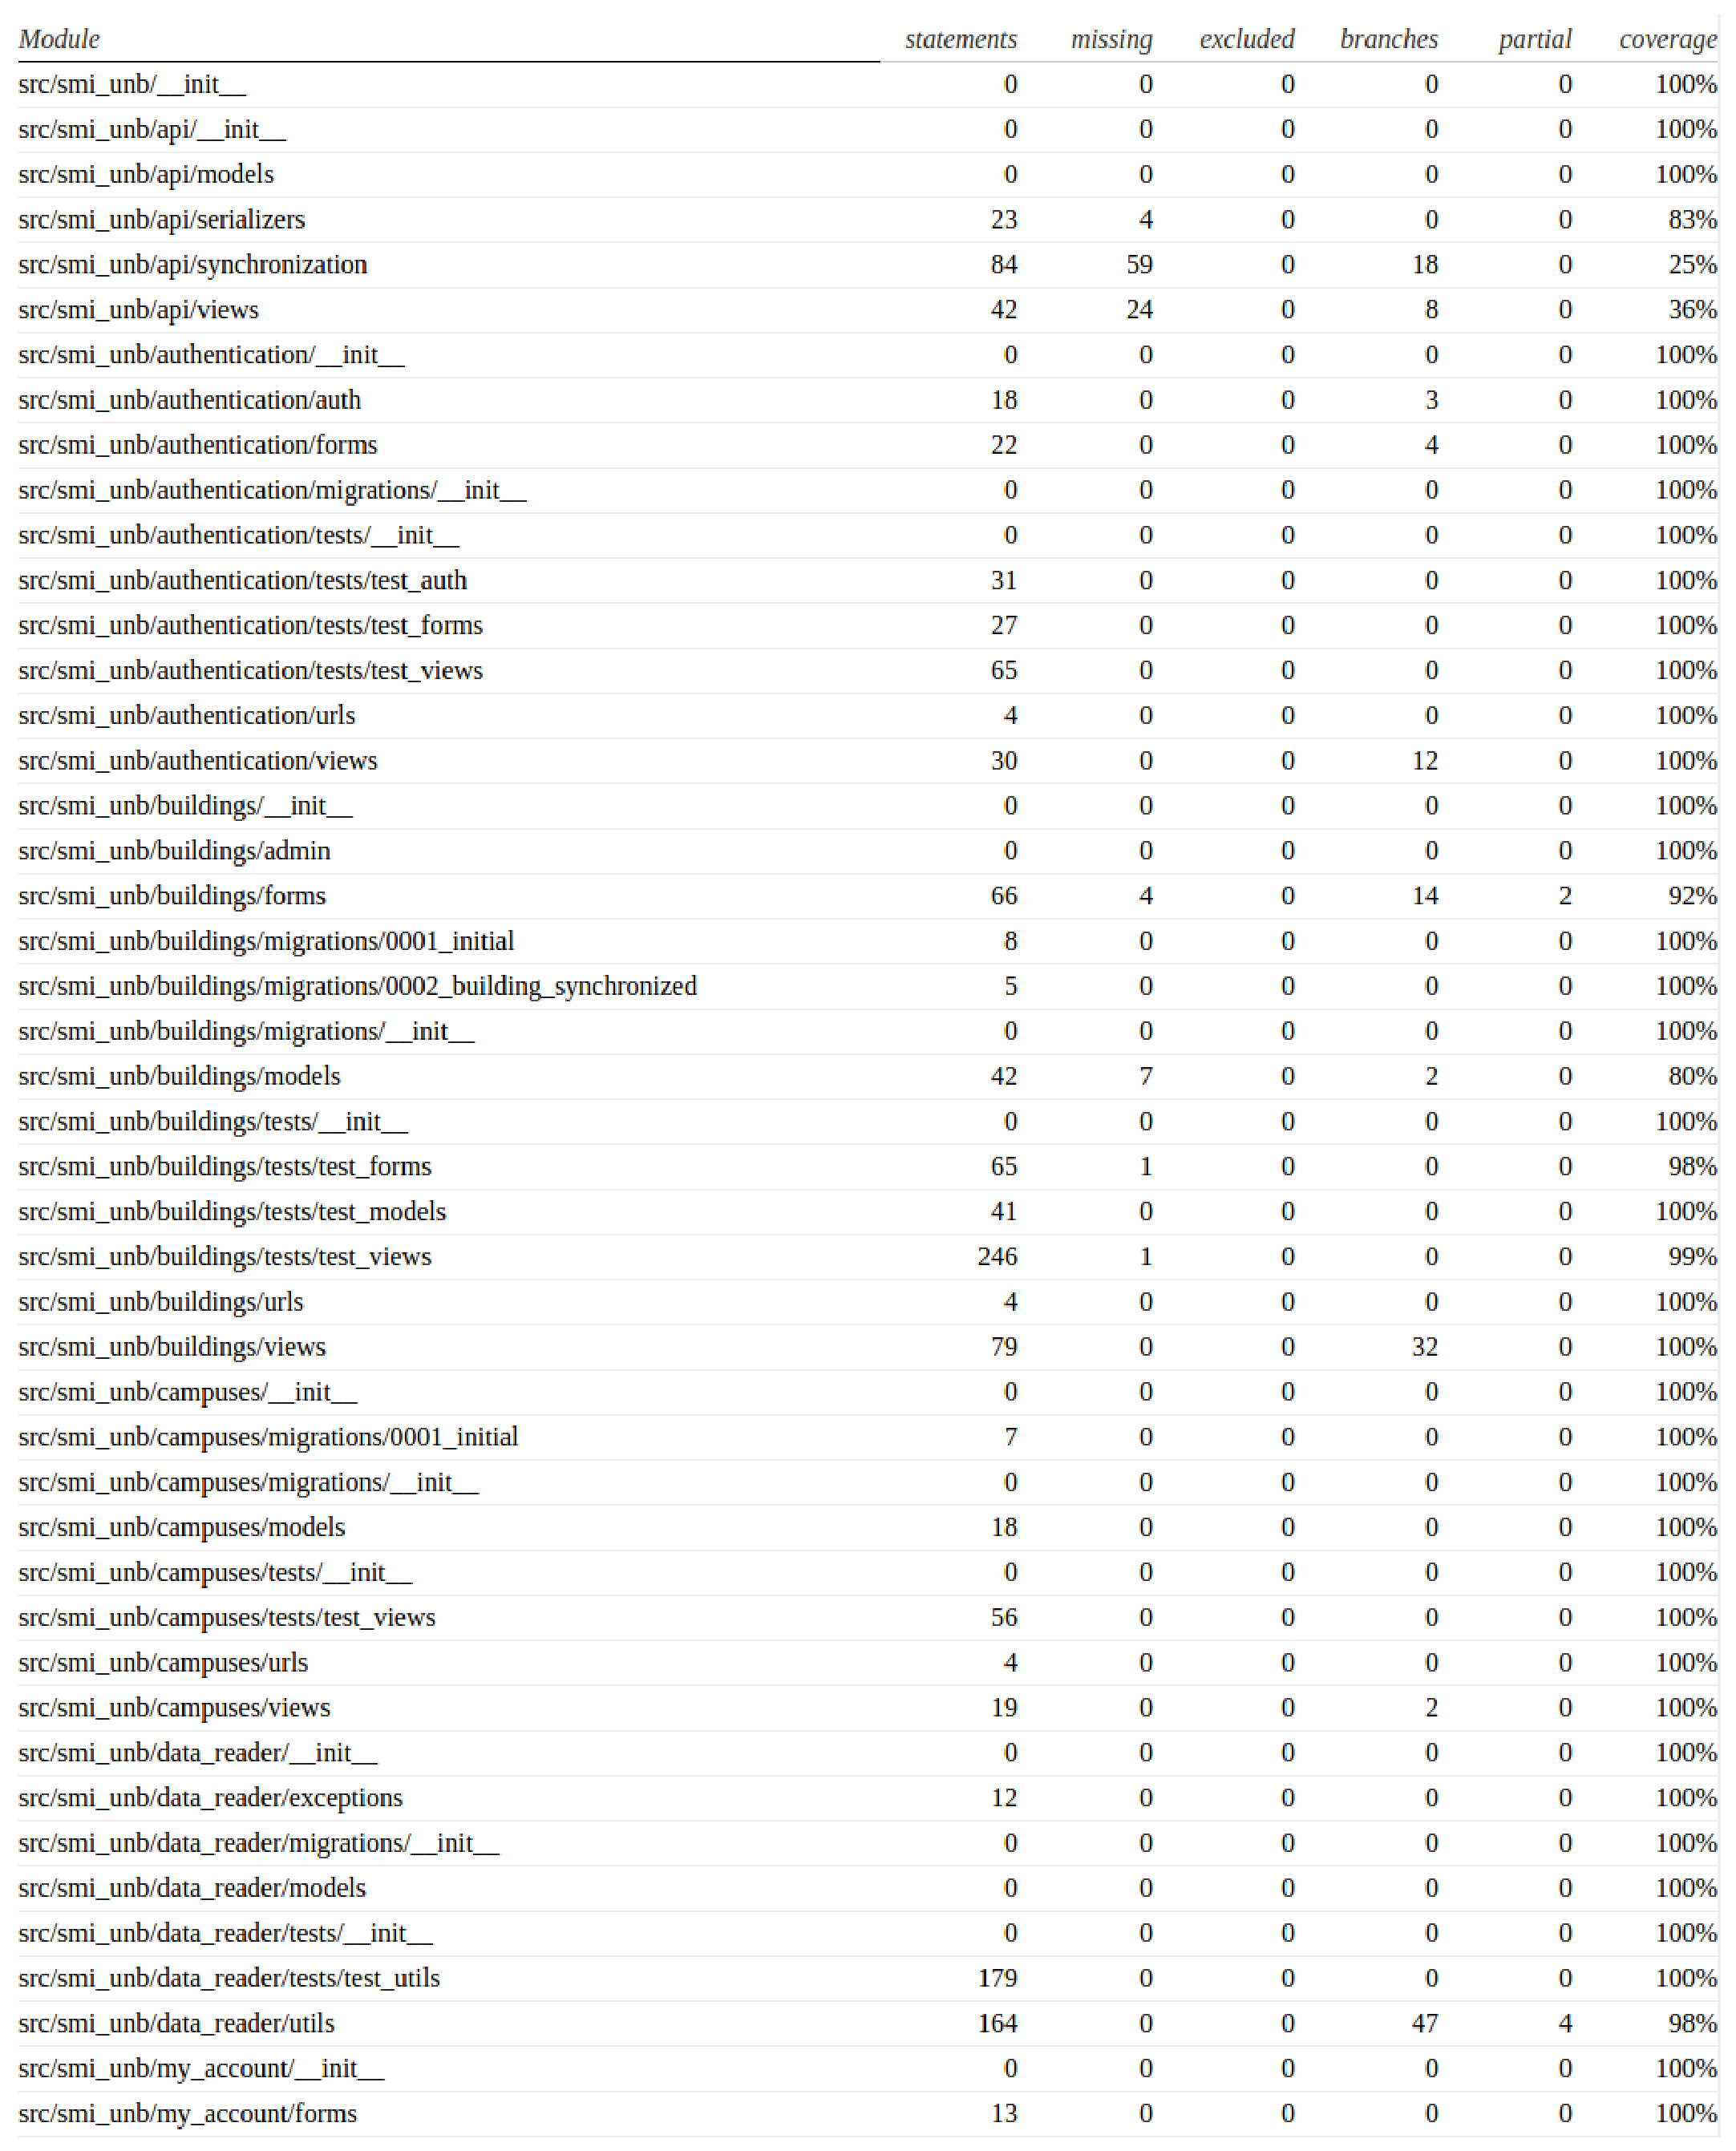
\includegraphics[keepaspectratio=true,scale=0.45]{figuras/cobertura01.eps}
    \caption{Primeira parte da cobertura do SMI-UnB.}
    \label{cobertura01}
\end{figure}

\begin{figure}[!htpb]
    \centering
    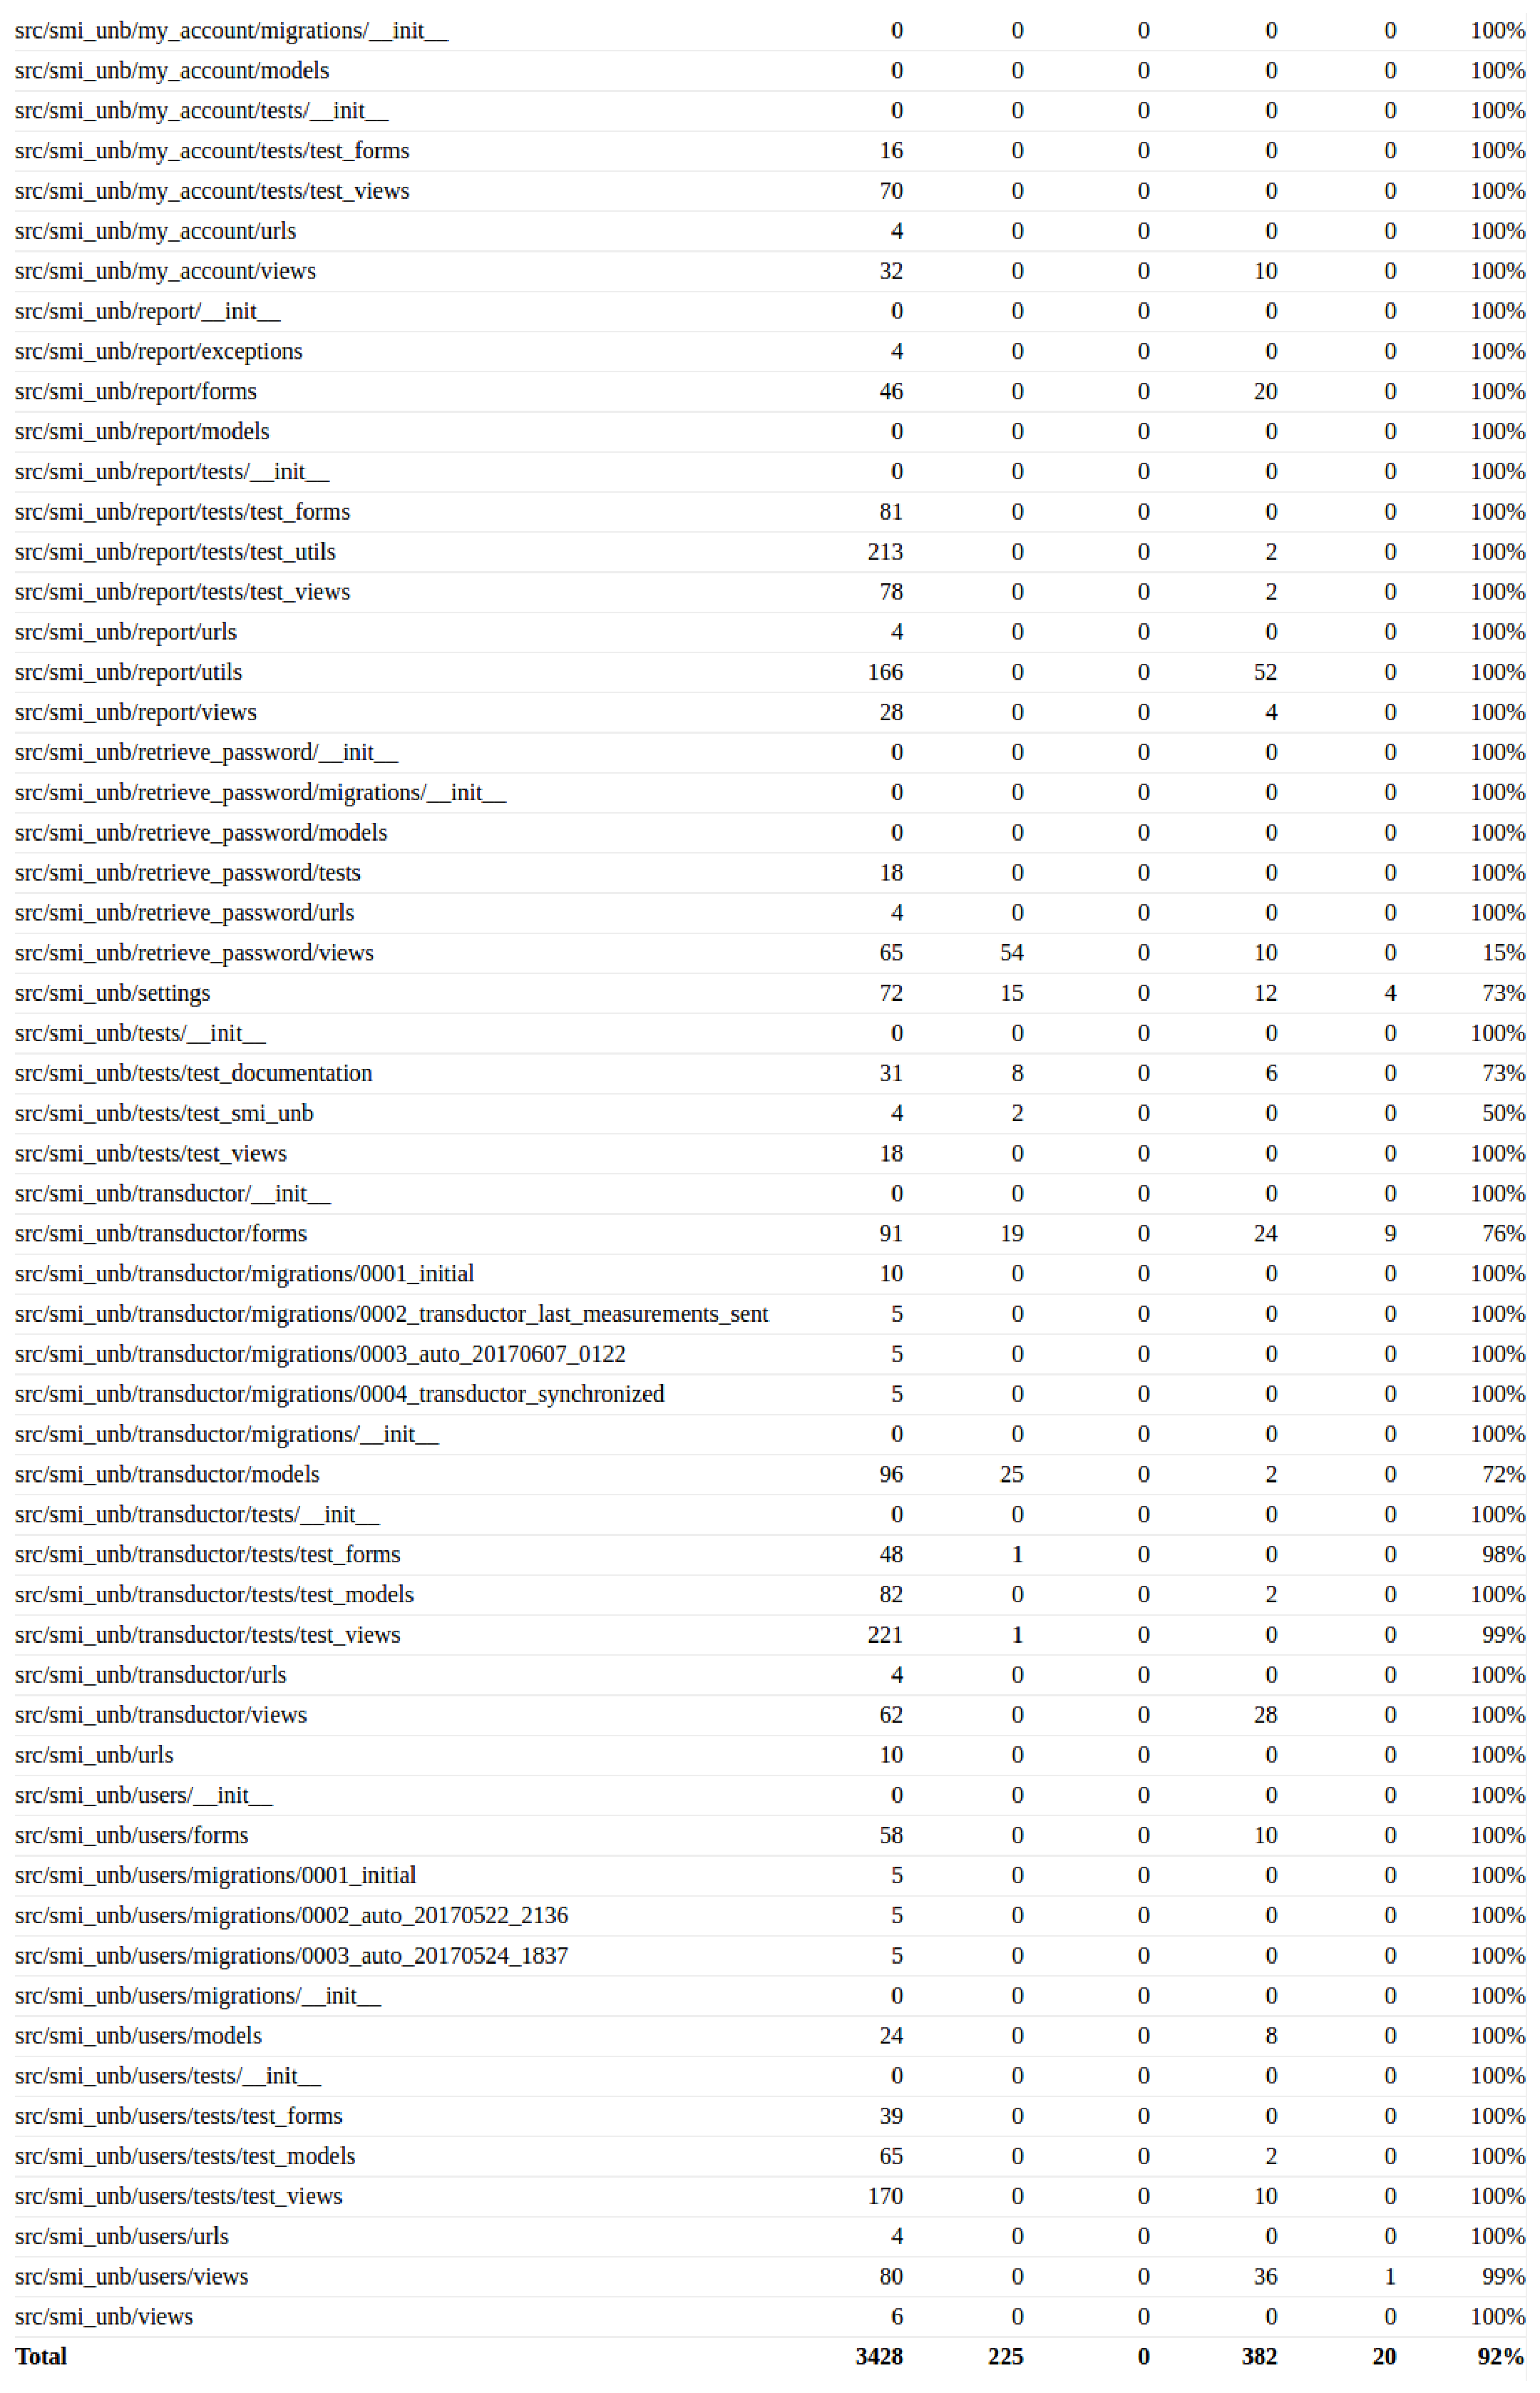
\includegraphics[keepaspectratio=true,scale=0.45]{figuras/cobertura02.eps}
    \caption{Segunda parte da cobertura do SMI-UnB.}
    \label{cobertura02}
\end{figure}

\chapter{Imagens da Aplicação}
\begin{figure}[!htpb]
    \centering
    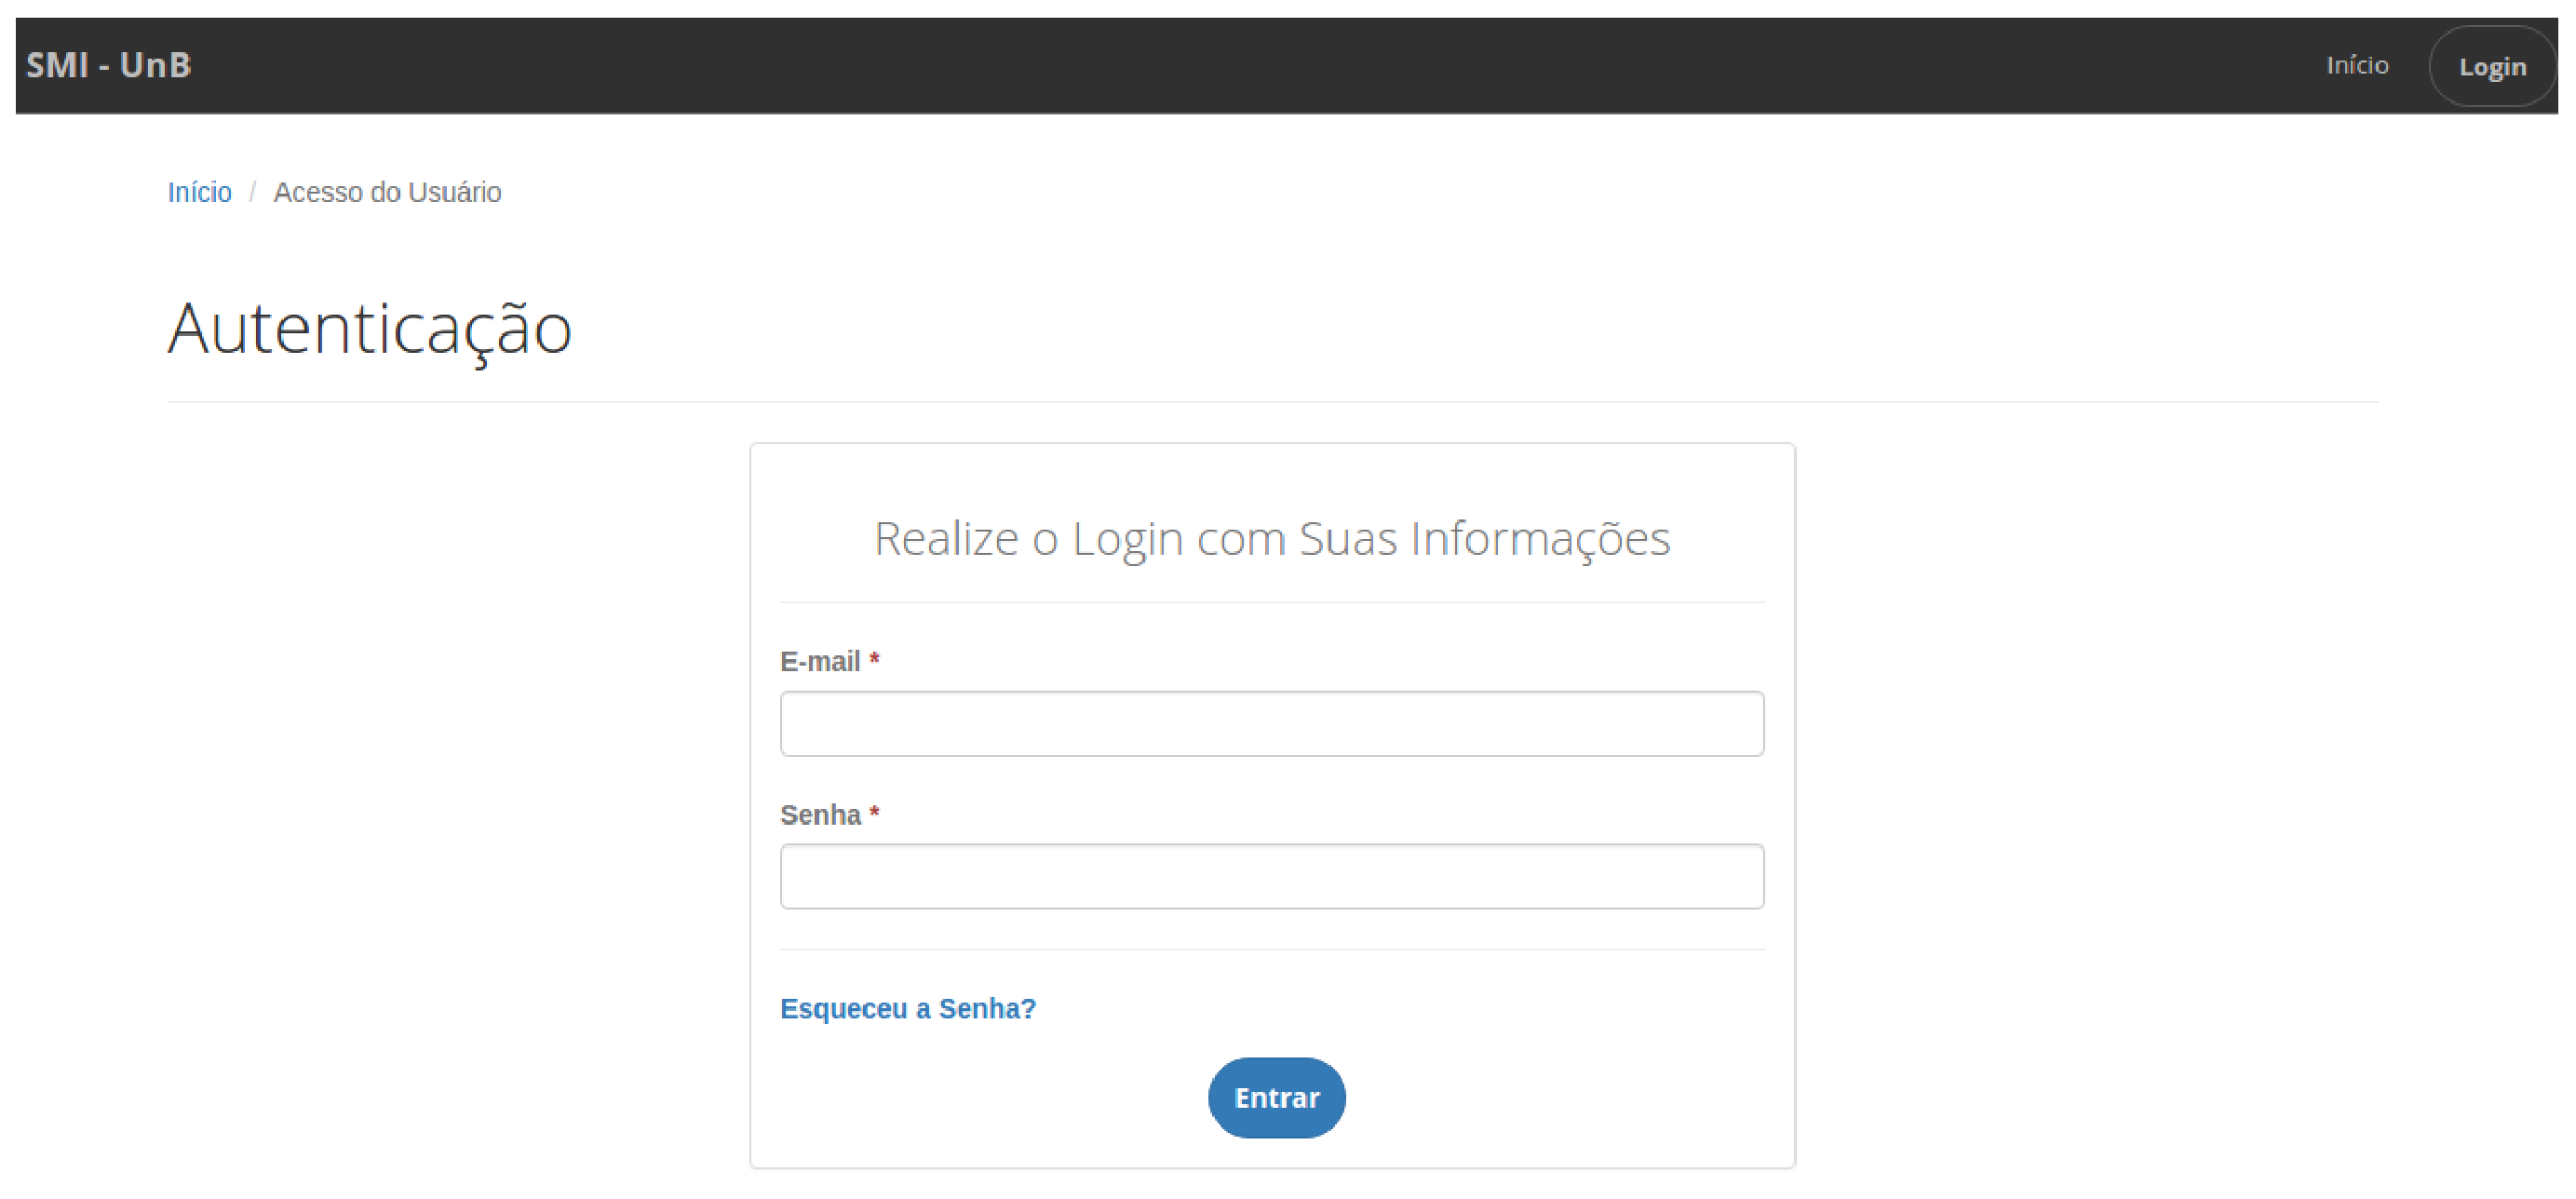
\includegraphics[keepaspectratio=true,scale=0.35]{figuras/img1.eps}
    \caption{Página de autenticação.}
    \label{img1}
\end{figure}

\begin{figure}[!htpb]
    \centering
    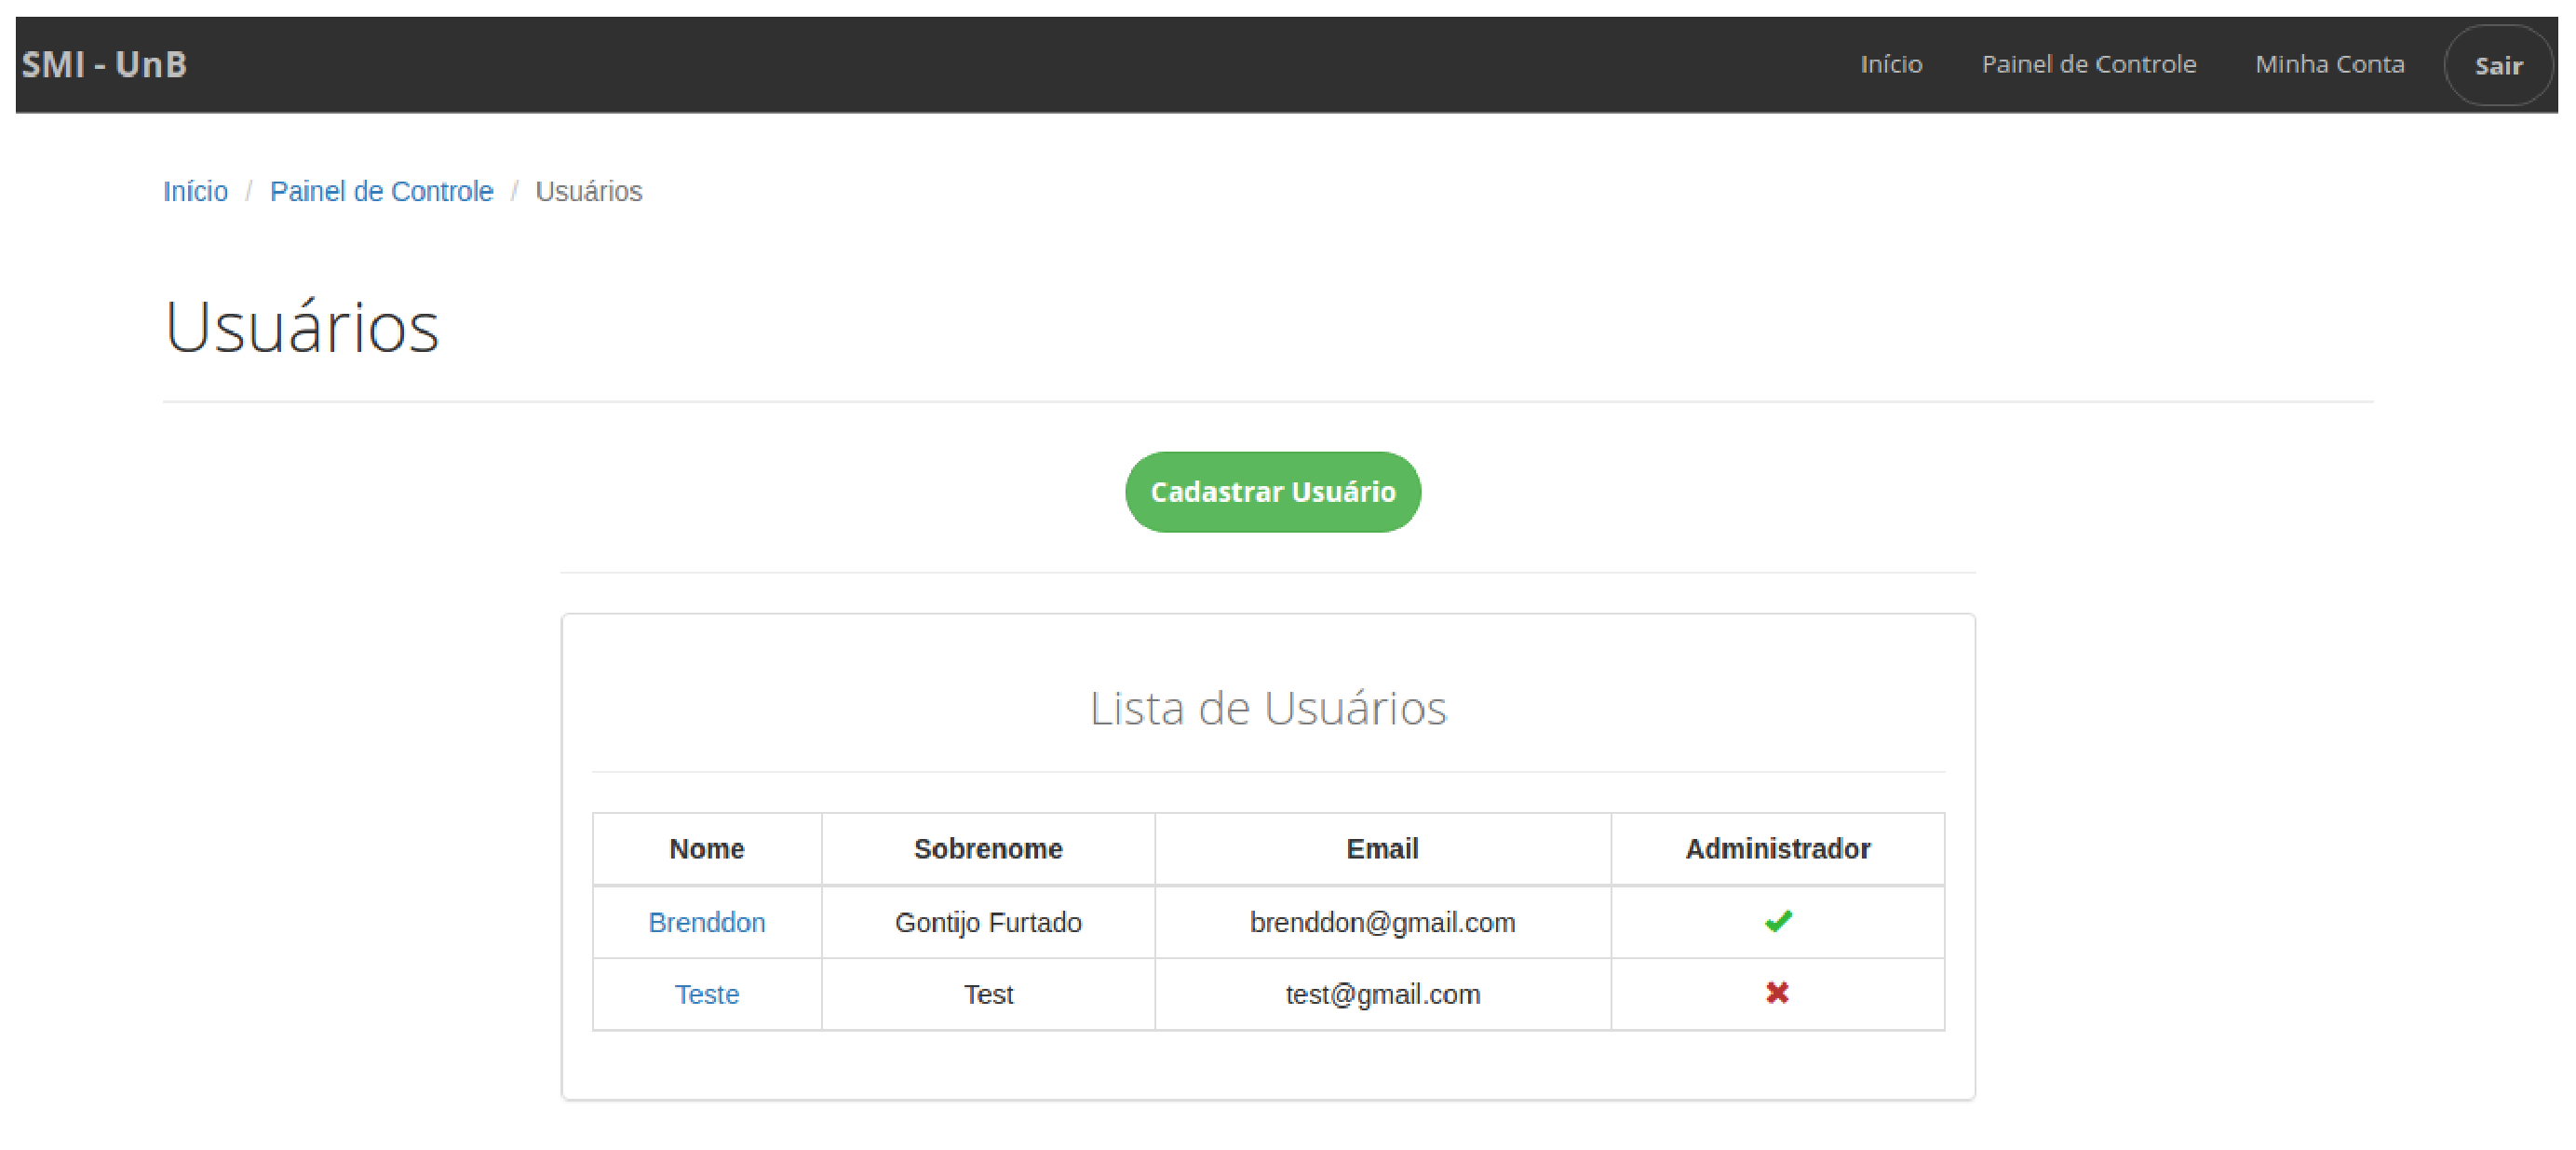
\includegraphics[keepaspectratio=true,scale=0.35]{figuras/img2.eps}
    \caption{Página de usuários.}
    \label{img2}
\end{figure}

\begin{figure}[!htpb]
    \centering
    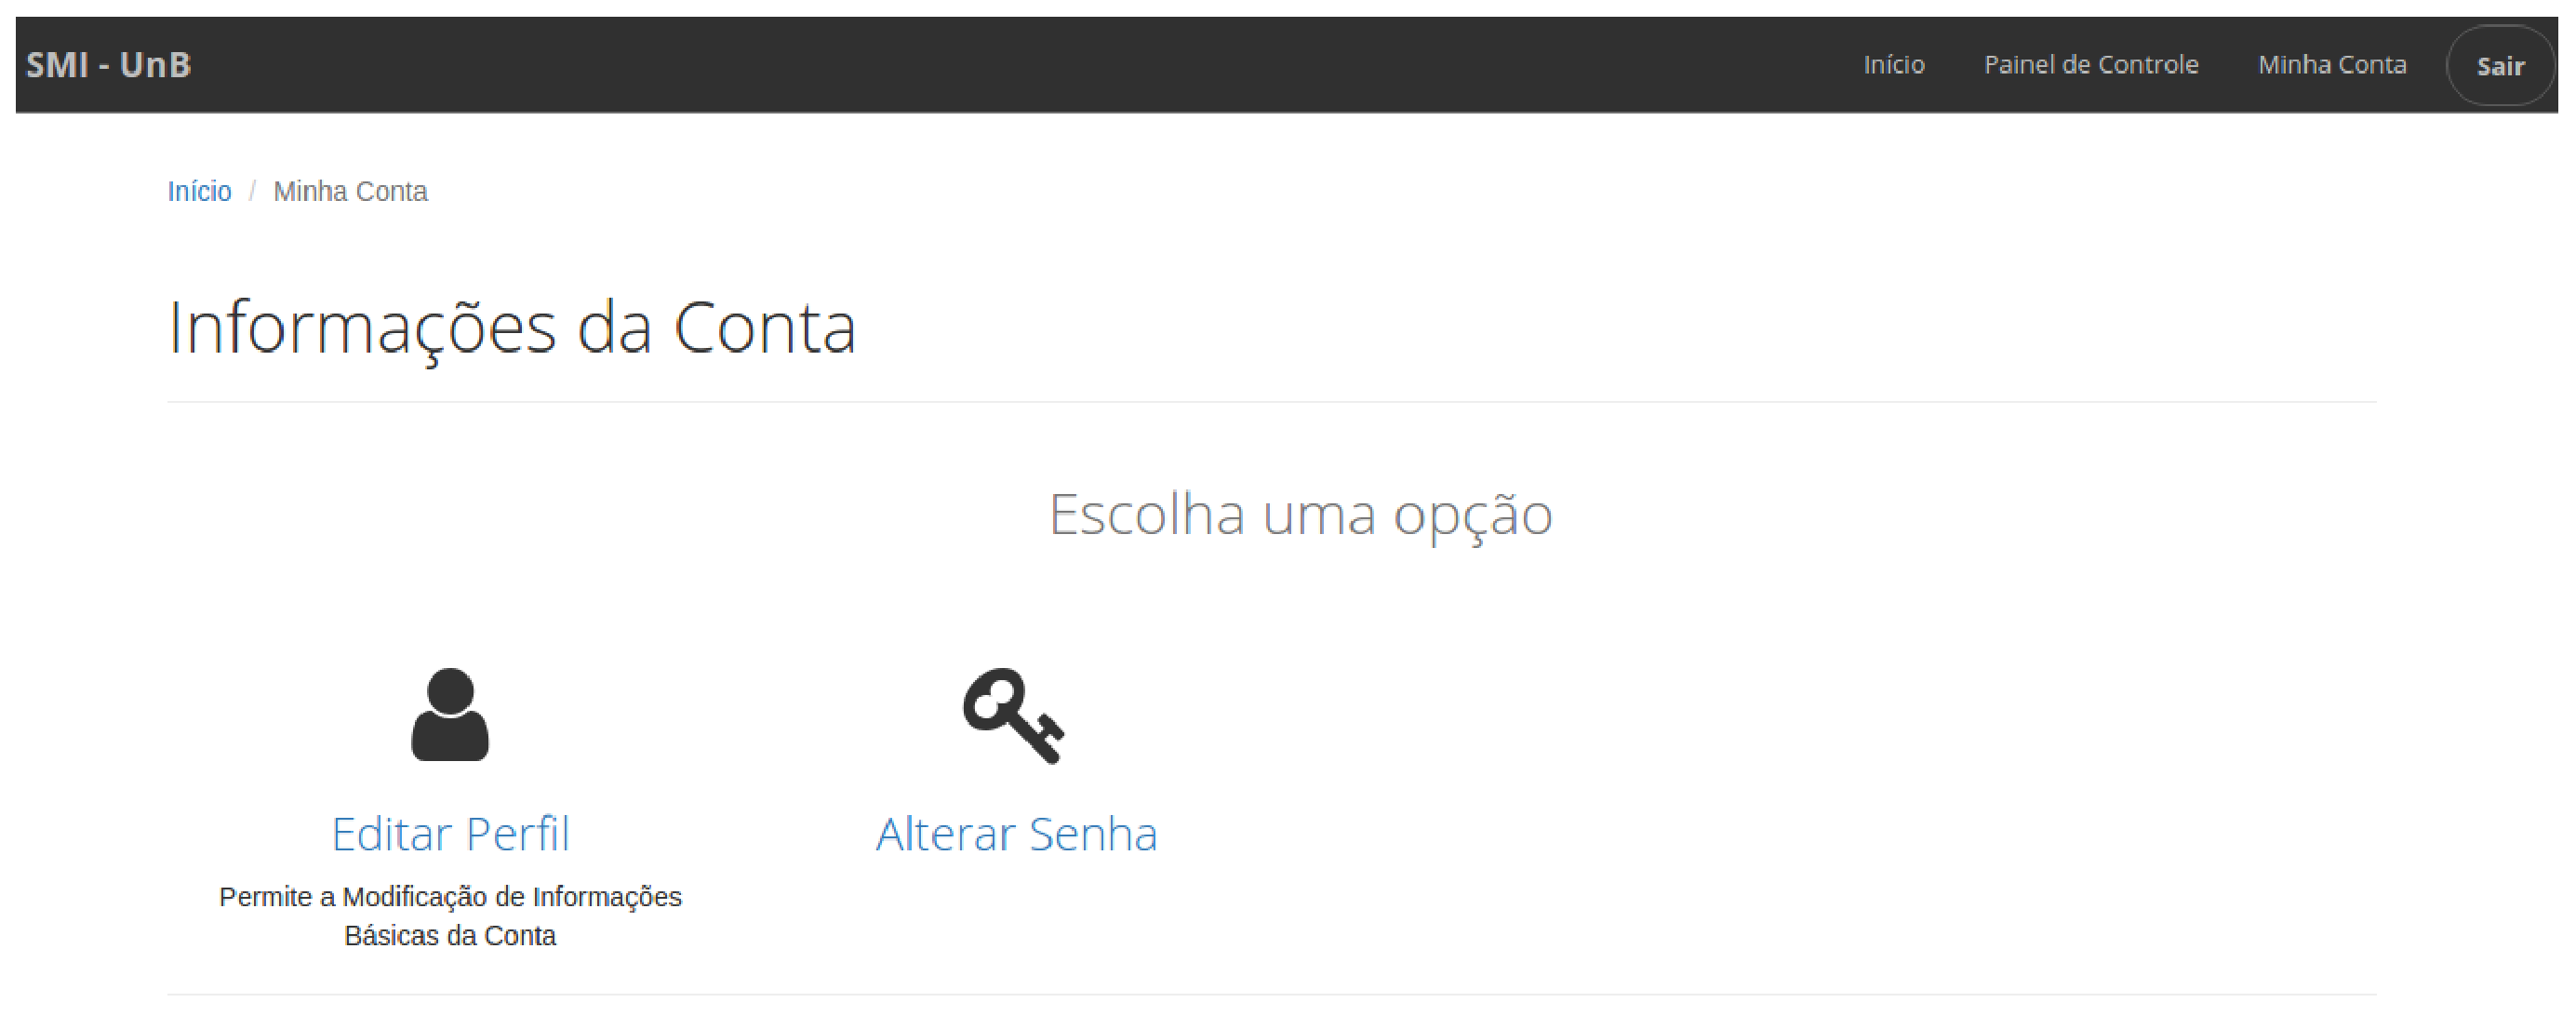
\includegraphics[keepaspectratio=true,scale=0.35]{figuras/img4.eps}
    \caption{Página de informações da conta.}
    \label{img4}
\end{figure}

\begin{figure}[!htpb]
    \centering
    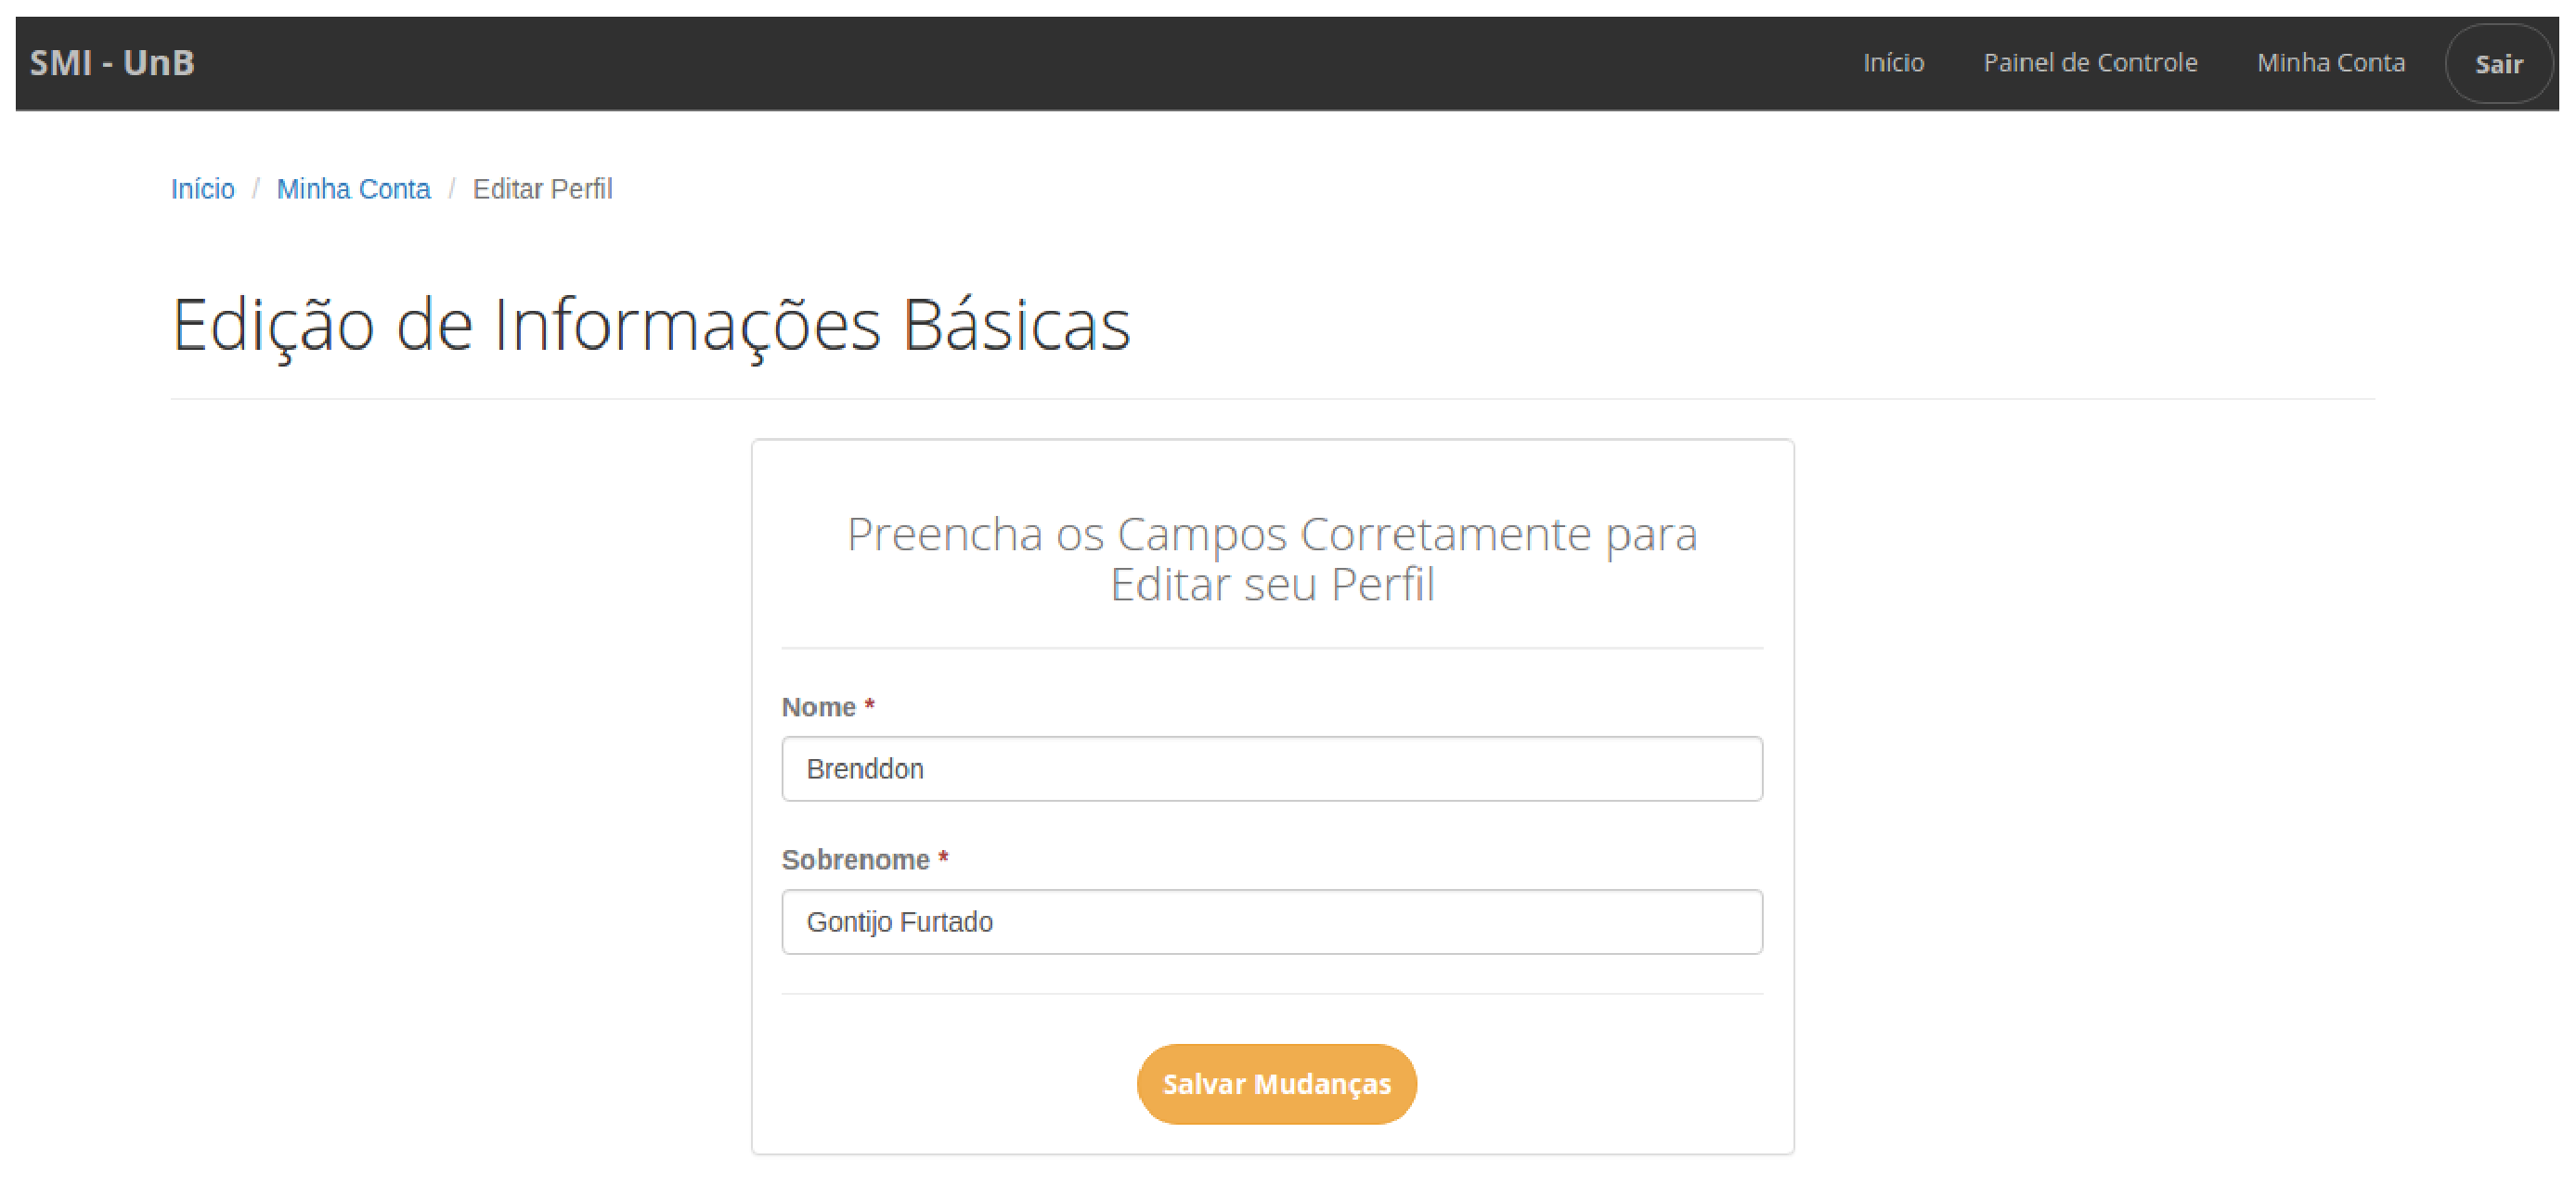
\includegraphics[keepaspectratio=true,scale=0.35]{figuras/img5.eps}
    \caption{Página de edição das informações básicas da conta.}
    \label{img5}
\end{figure}

\begin{figure}[!htpb]
    \centering
    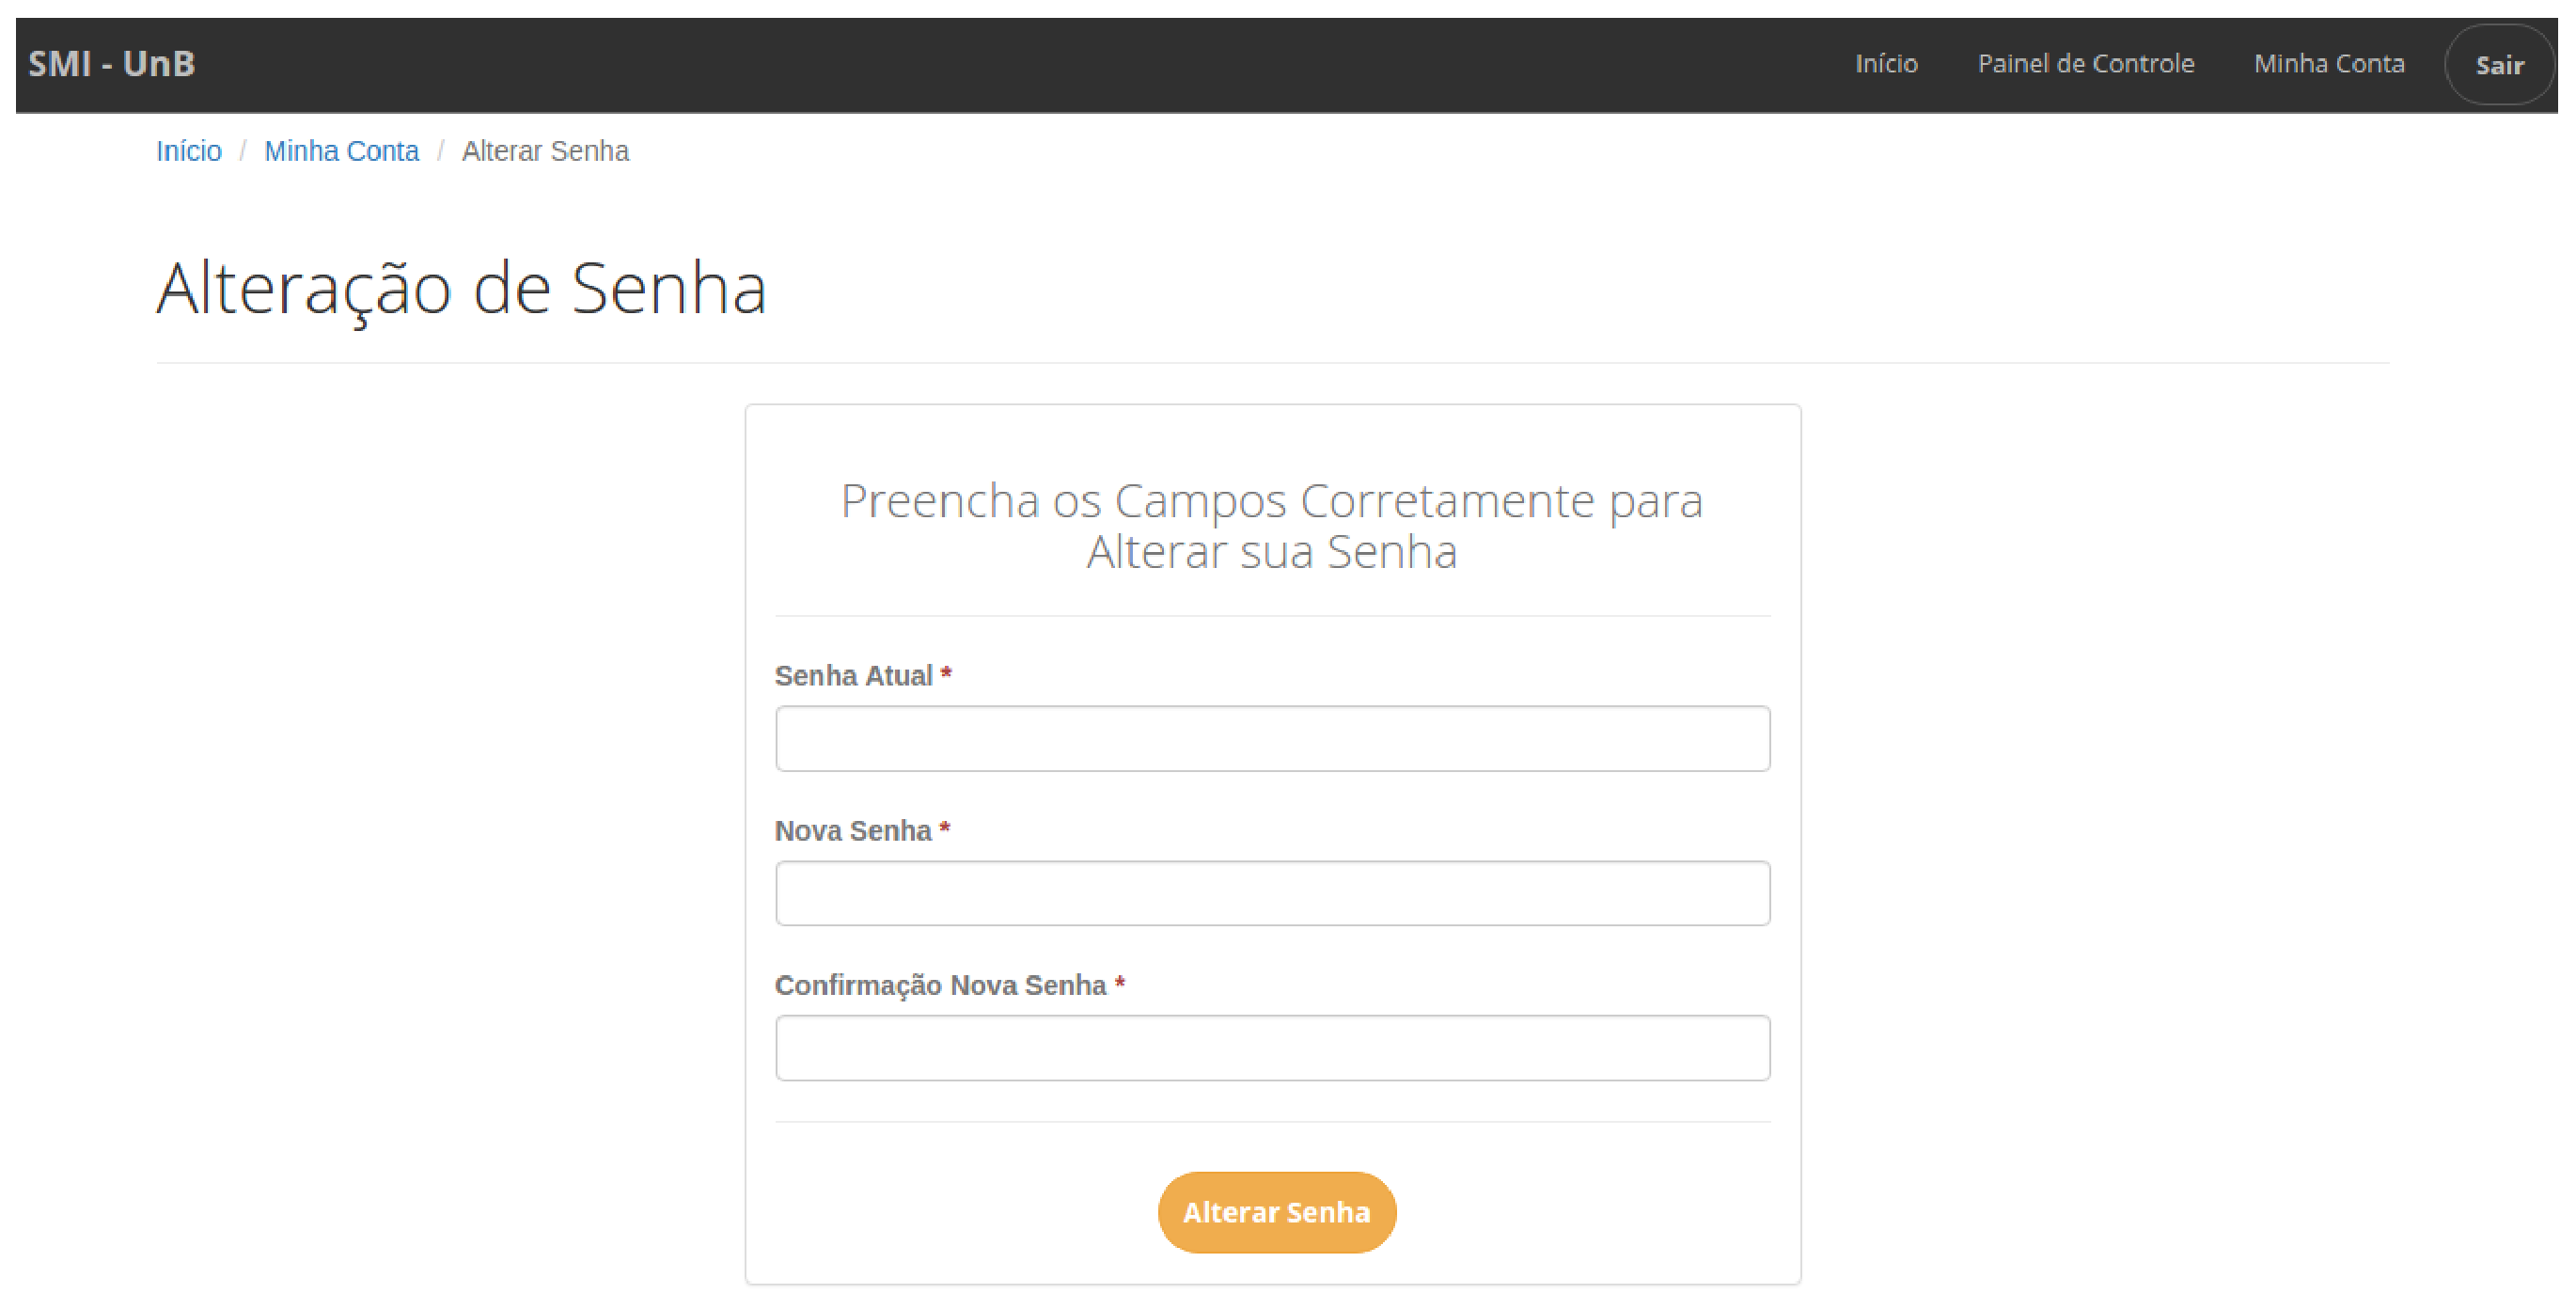
\includegraphics[keepaspectratio=true,scale=0.35]{figuras/img6.eps}
    \caption{Página de alteração de senha.}
    \label{img6}
\end{figure}

\begin{figure}[!htpb]
    \centering
    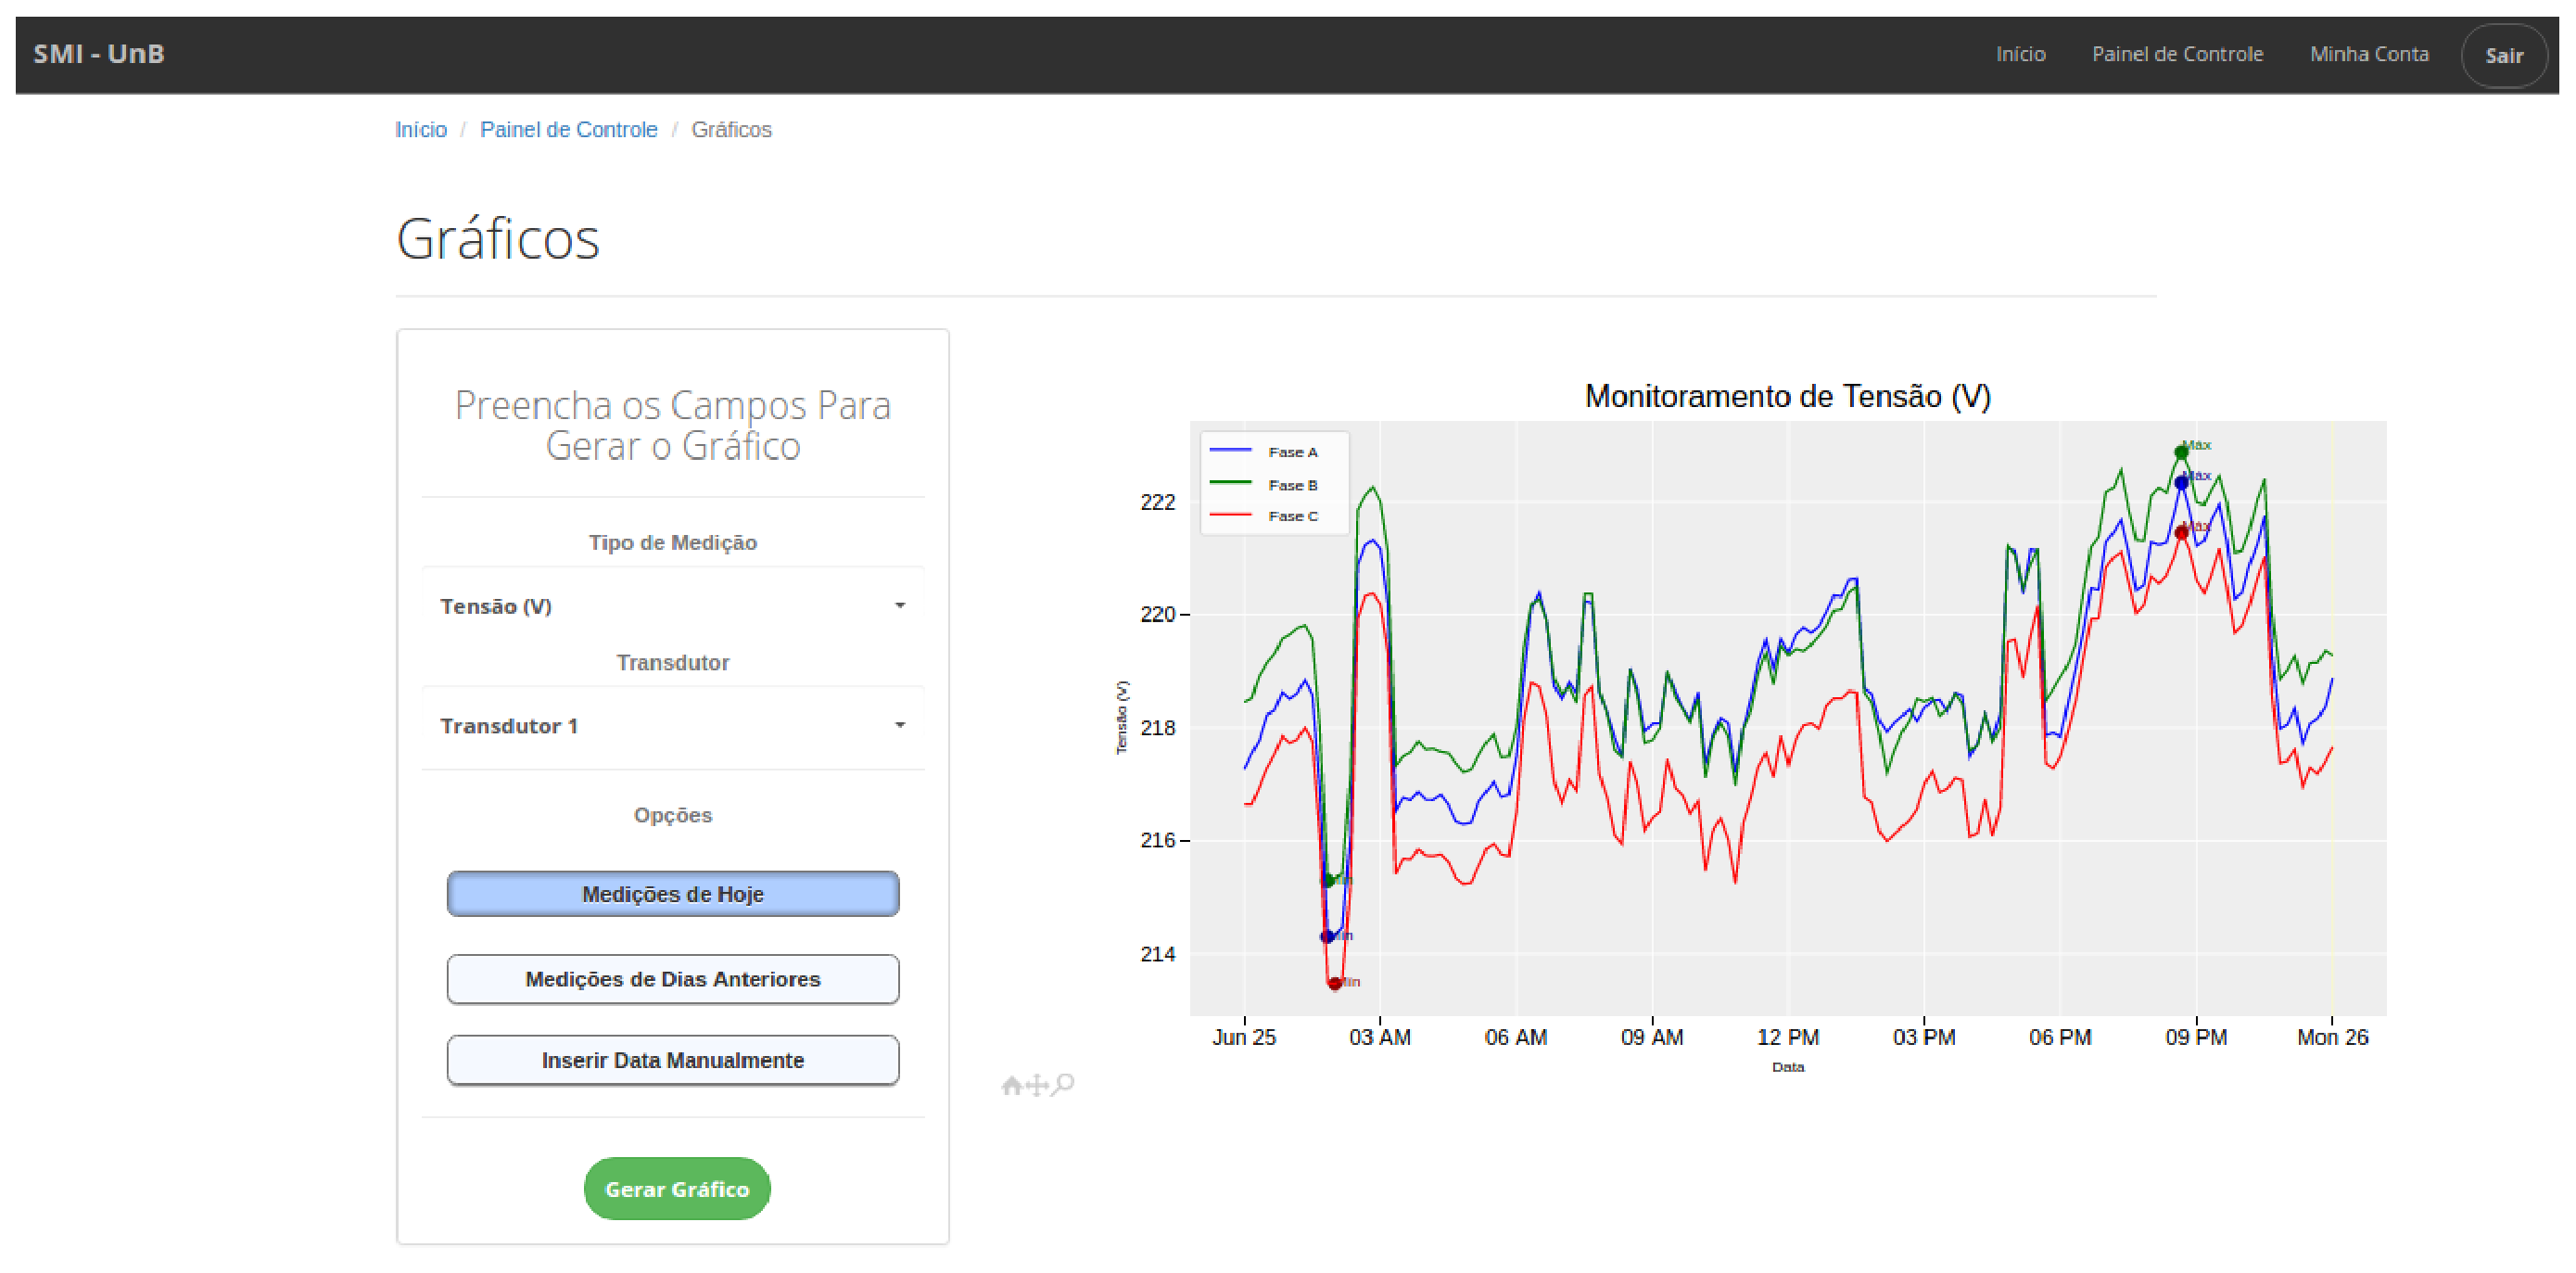
\includegraphics[keepaspectratio=true,scale=0.35]{figuras/img15.eps}
    \caption{Página de gráficos.}
    \label{img15}
\end{figure}

\begin{figure}[!htpb]
    \centering
    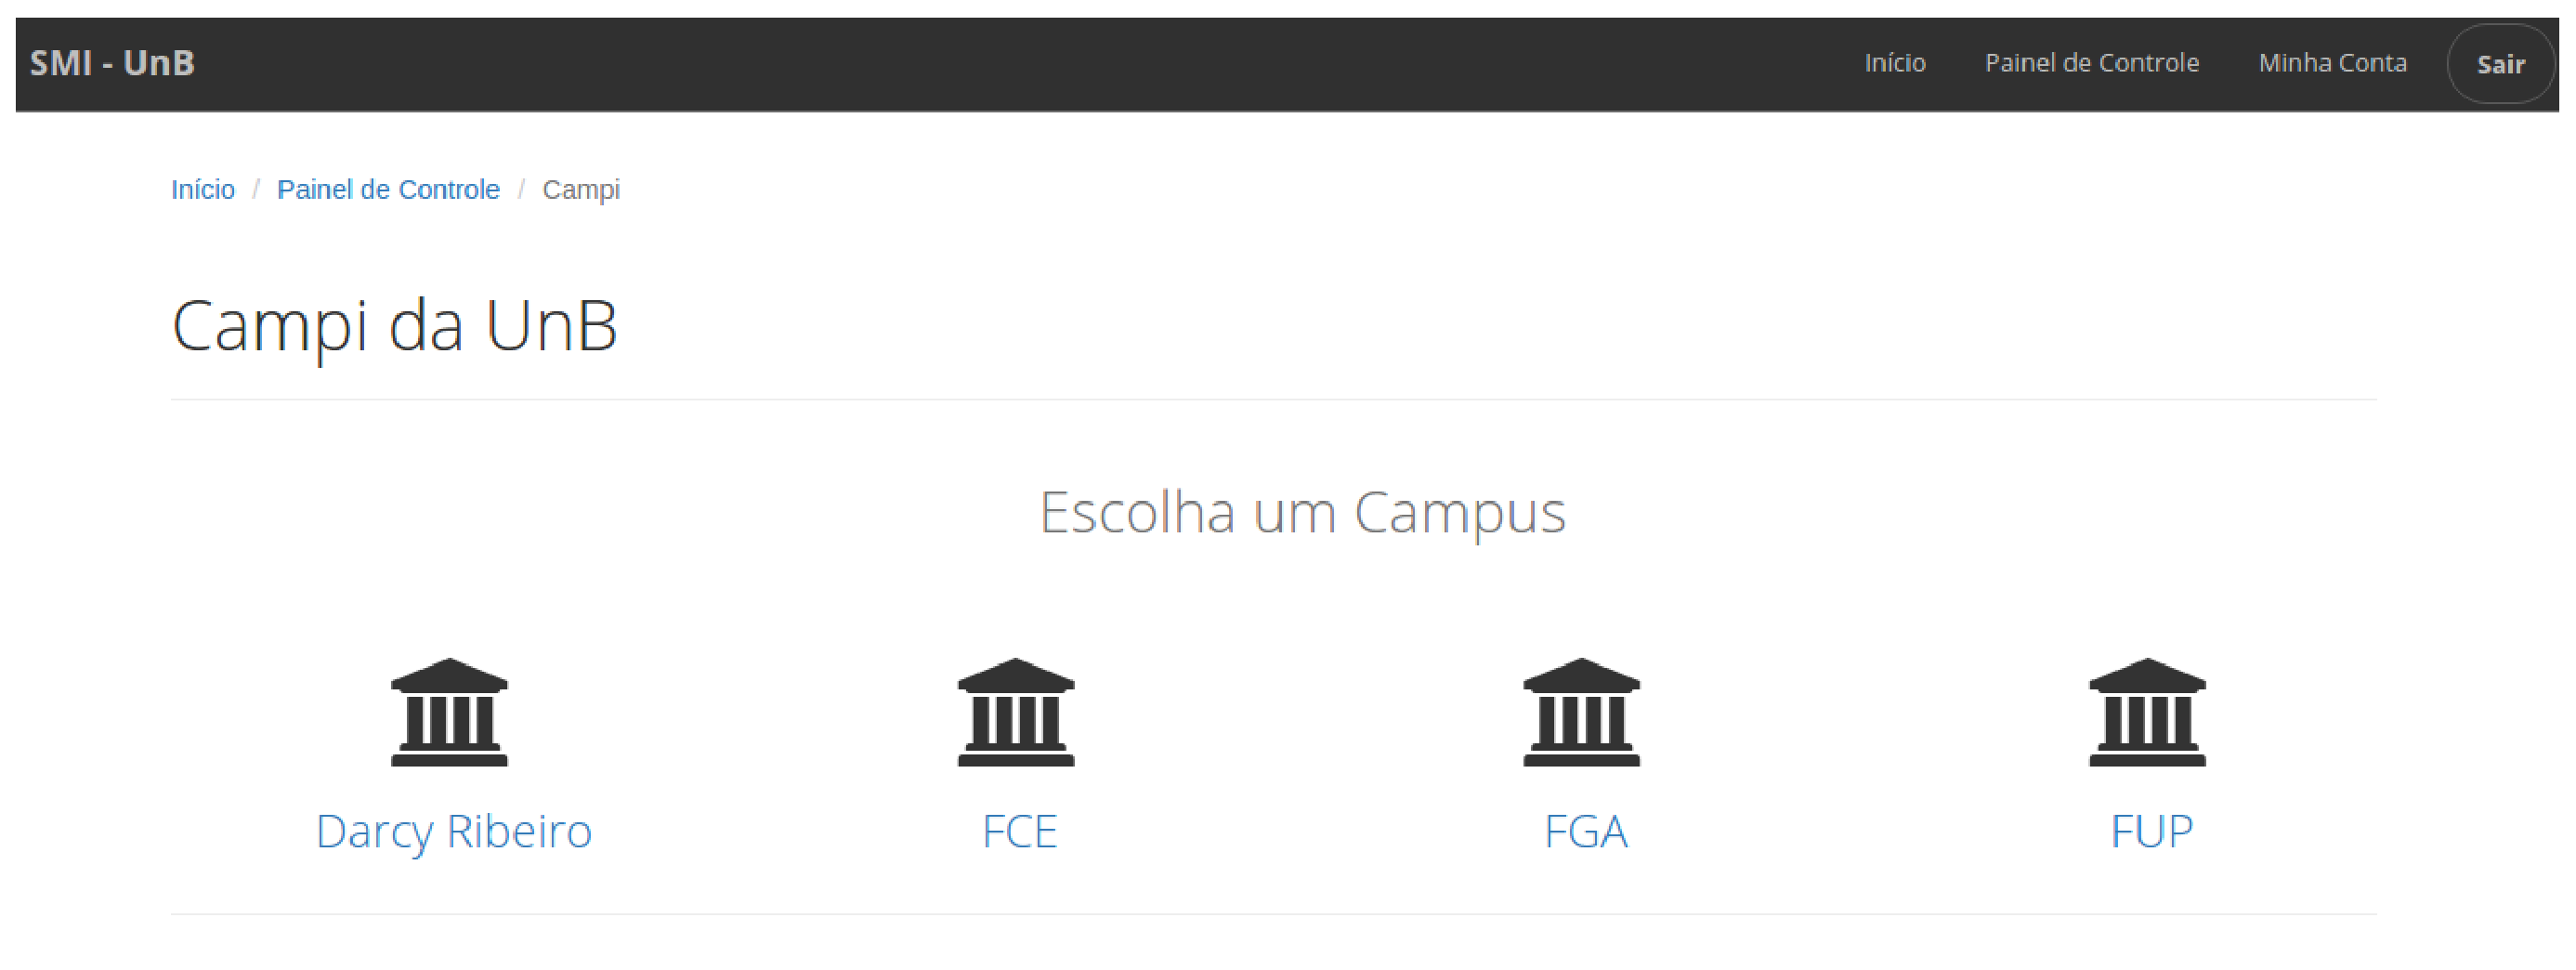
\includegraphics[keepaspectratio=true,scale=0.35]{figuras/img7.eps}
    \caption{Página dos câmpus da UnB.}
    \label{img7}
\end{figure}

\begin{figure}[!htpb]
    \centering
    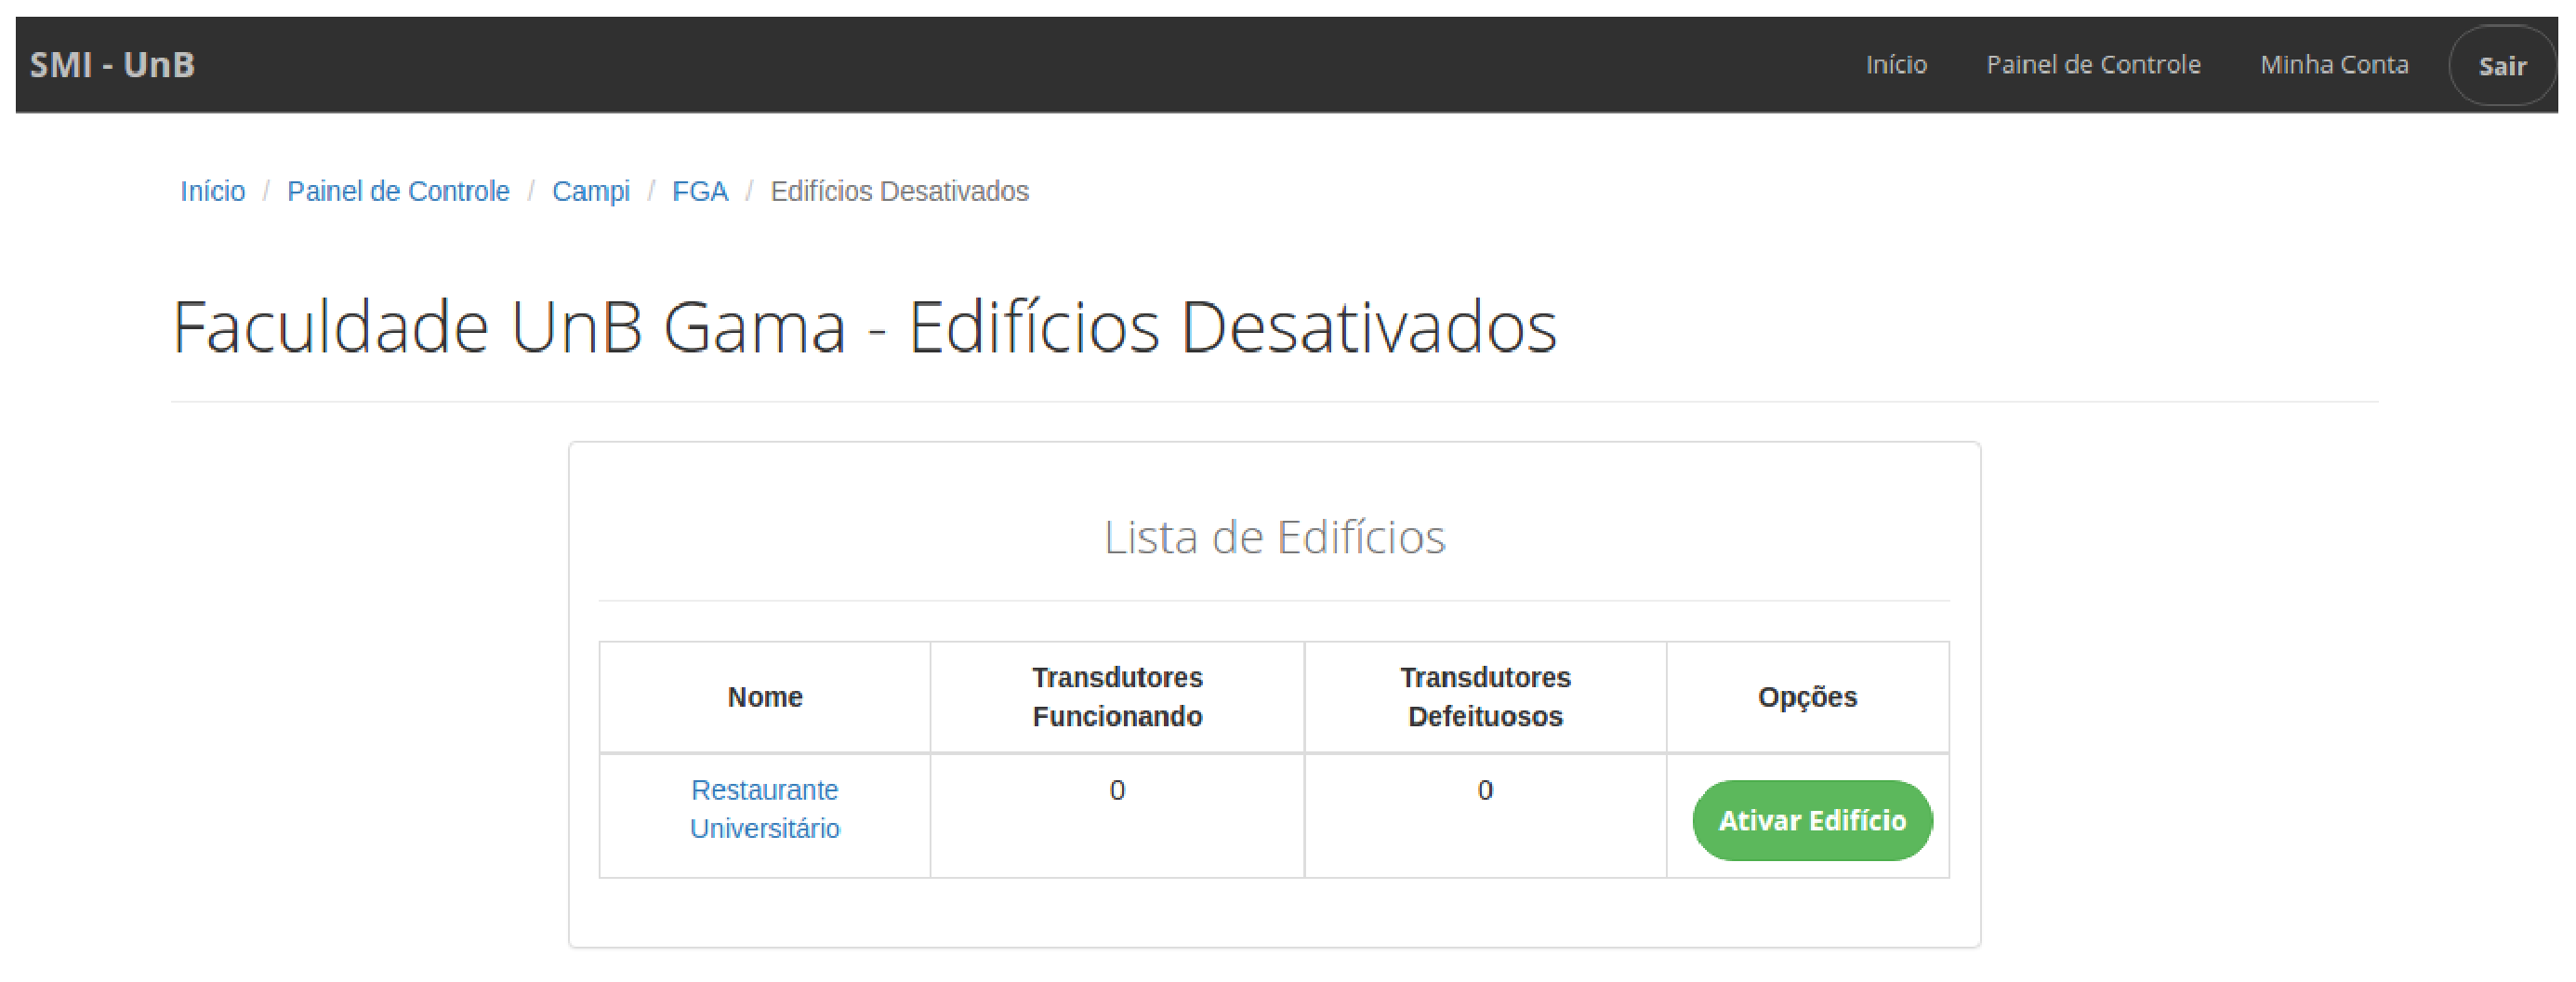
\includegraphics[keepaspectratio=true,scale=0.35]{figuras/img8.eps}
    \caption{Página de edifícios desativados em um campus.}
    \label{img8}
\end{figure}

\begin{figure}[!htpb]
    \centering
    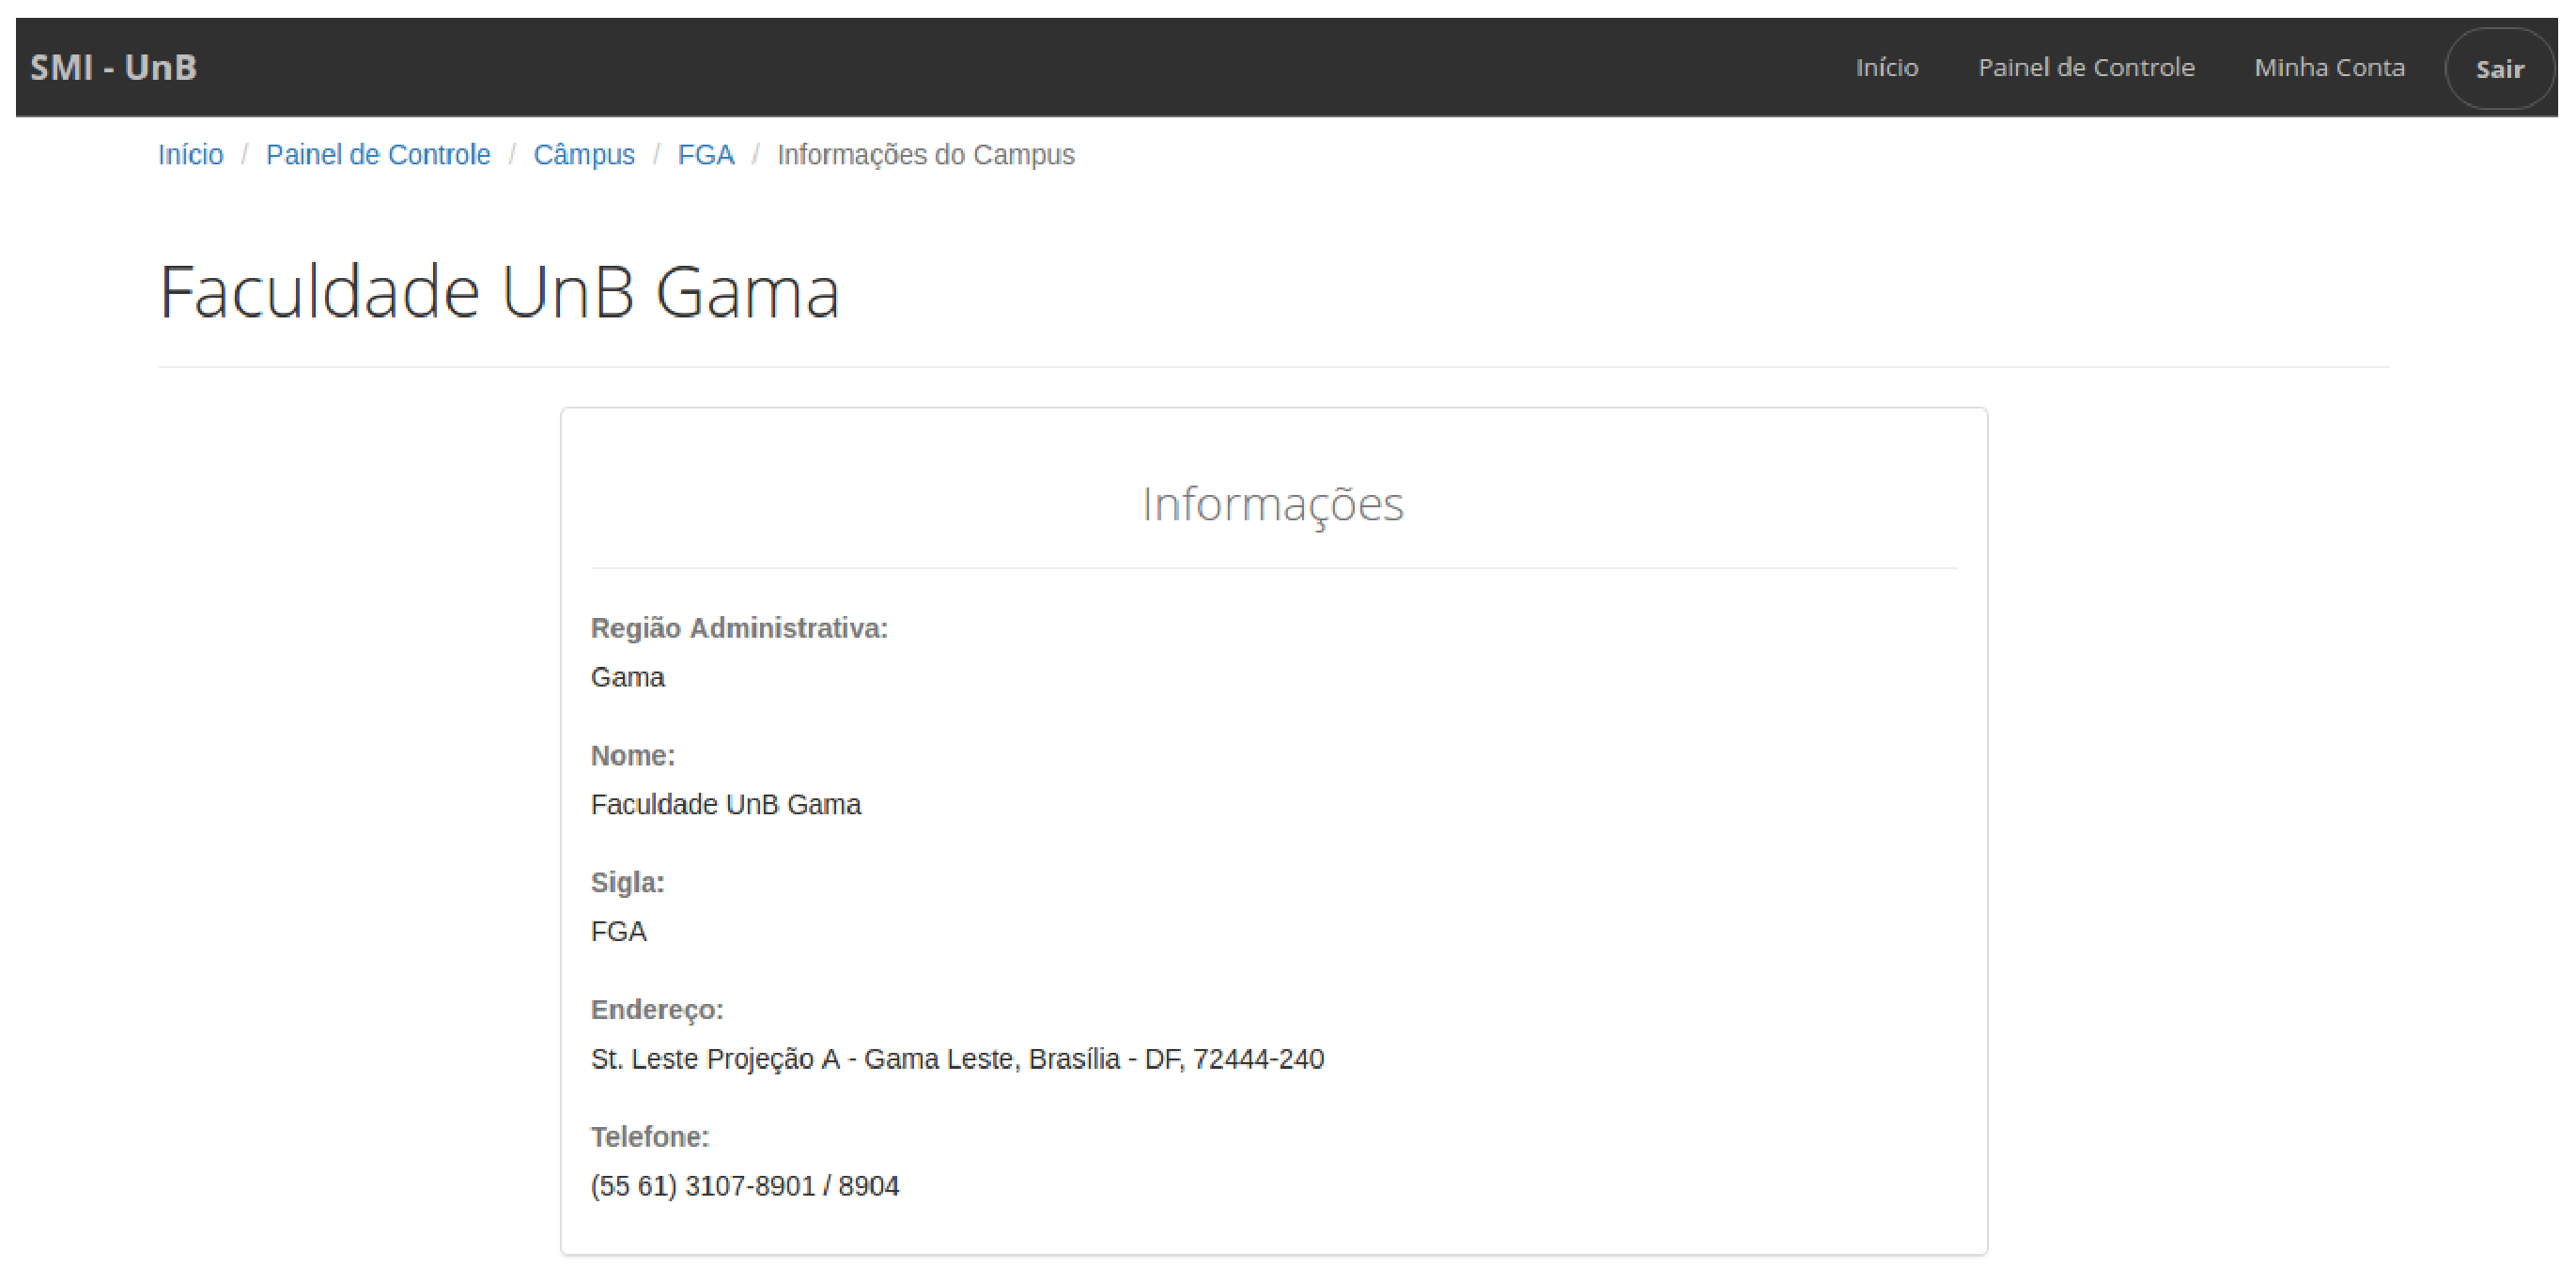
\includegraphics[keepaspectratio=true,scale=0.35]{figuras/img9.eps}
    \caption{Página de informações de em um campus.}
    \label{img9}
\end{figure}

\begin{figure}[!htpb]
    \centering
    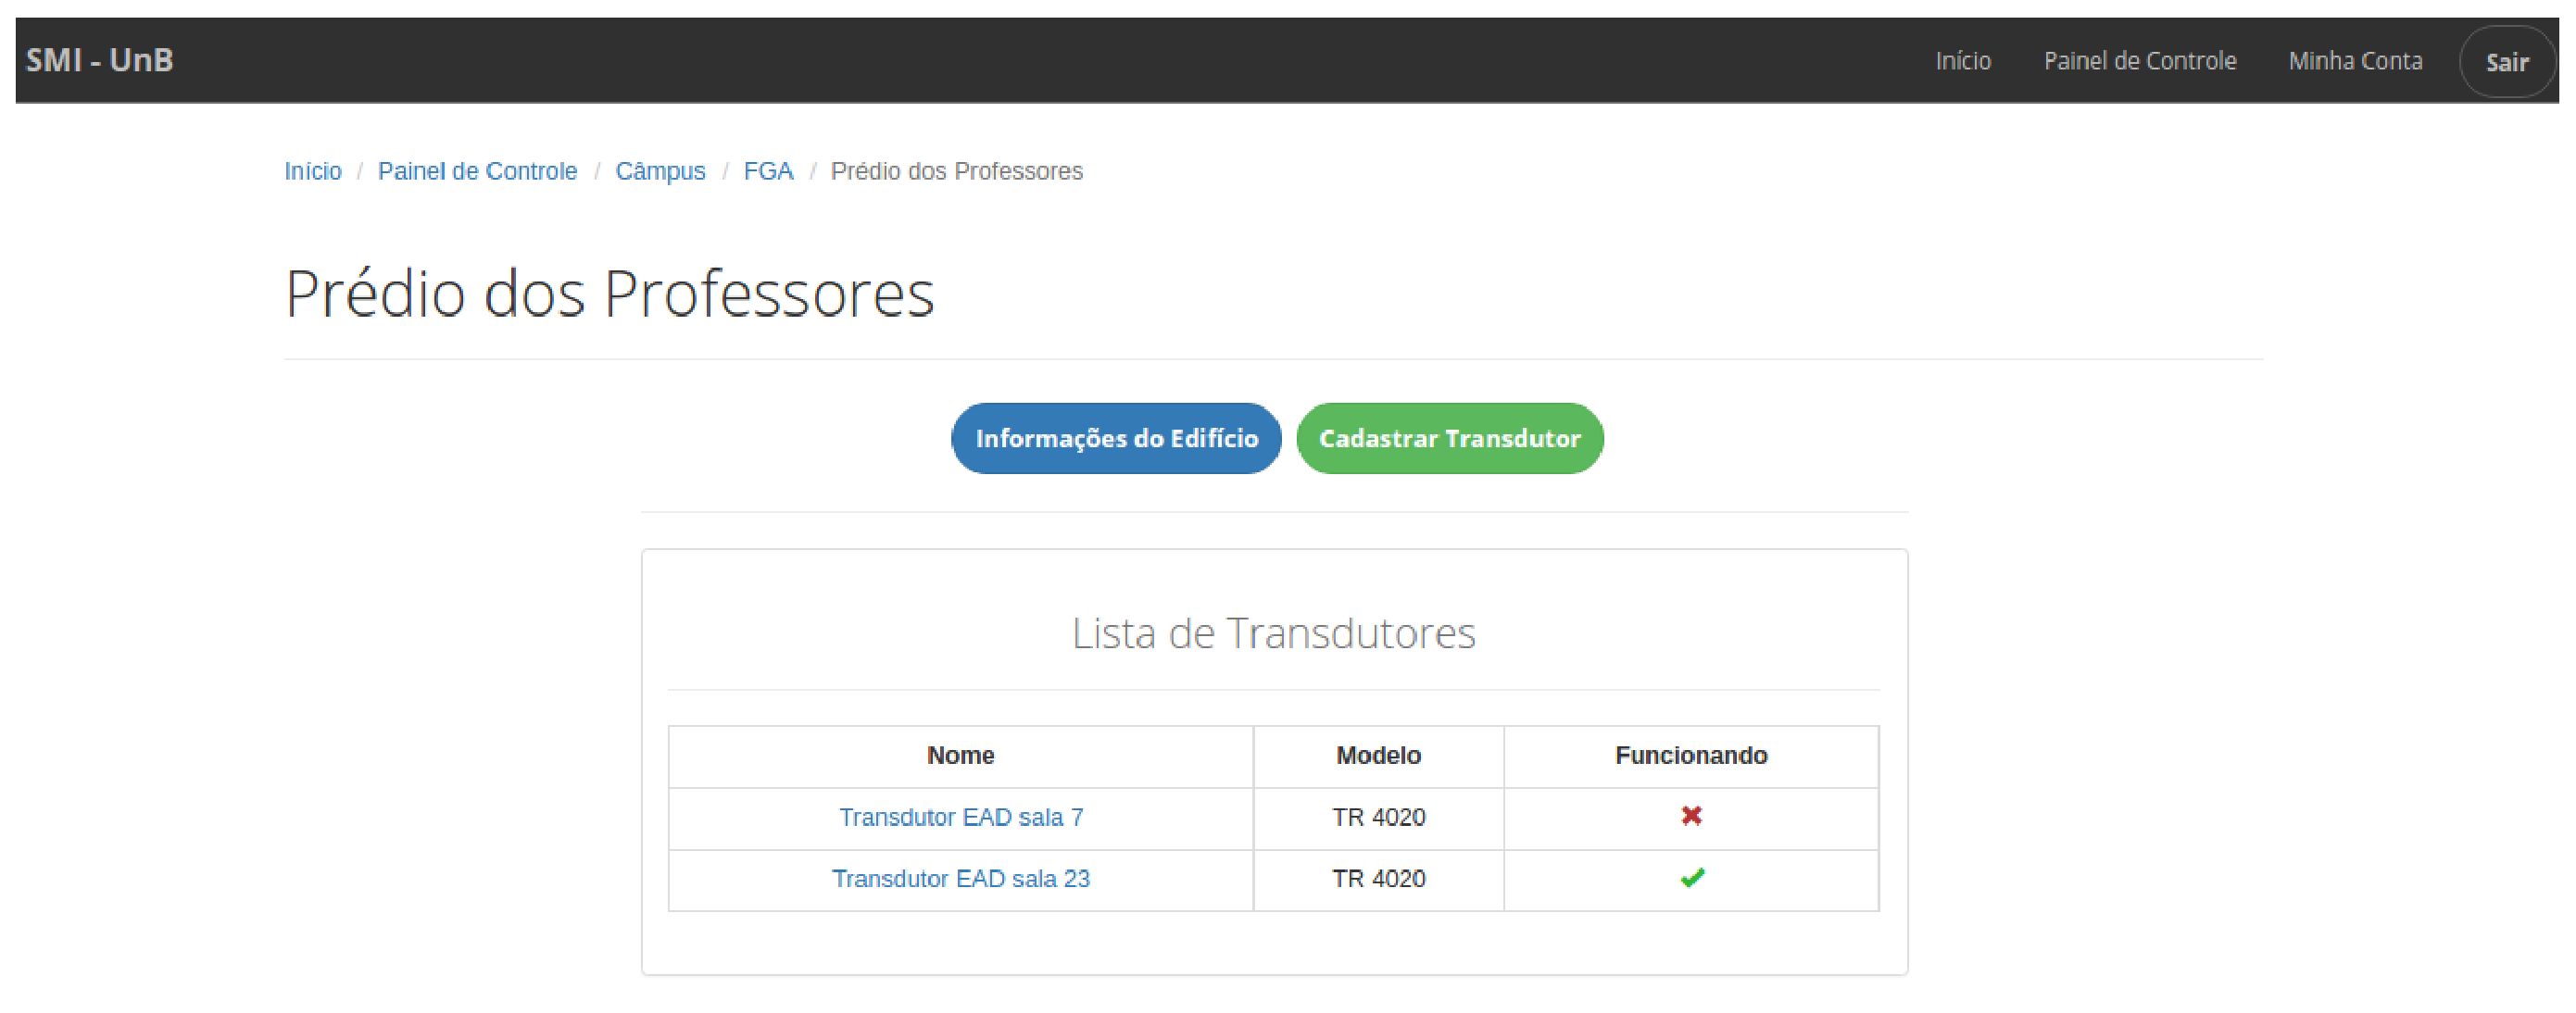
\includegraphics[keepaspectratio=true,scale=0.35]{figuras/img11.eps}
    \caption{Página principal de um edifício.}
    \label{img11}
\end{figure}

\begin{figure}[!htpb]
    \centering
    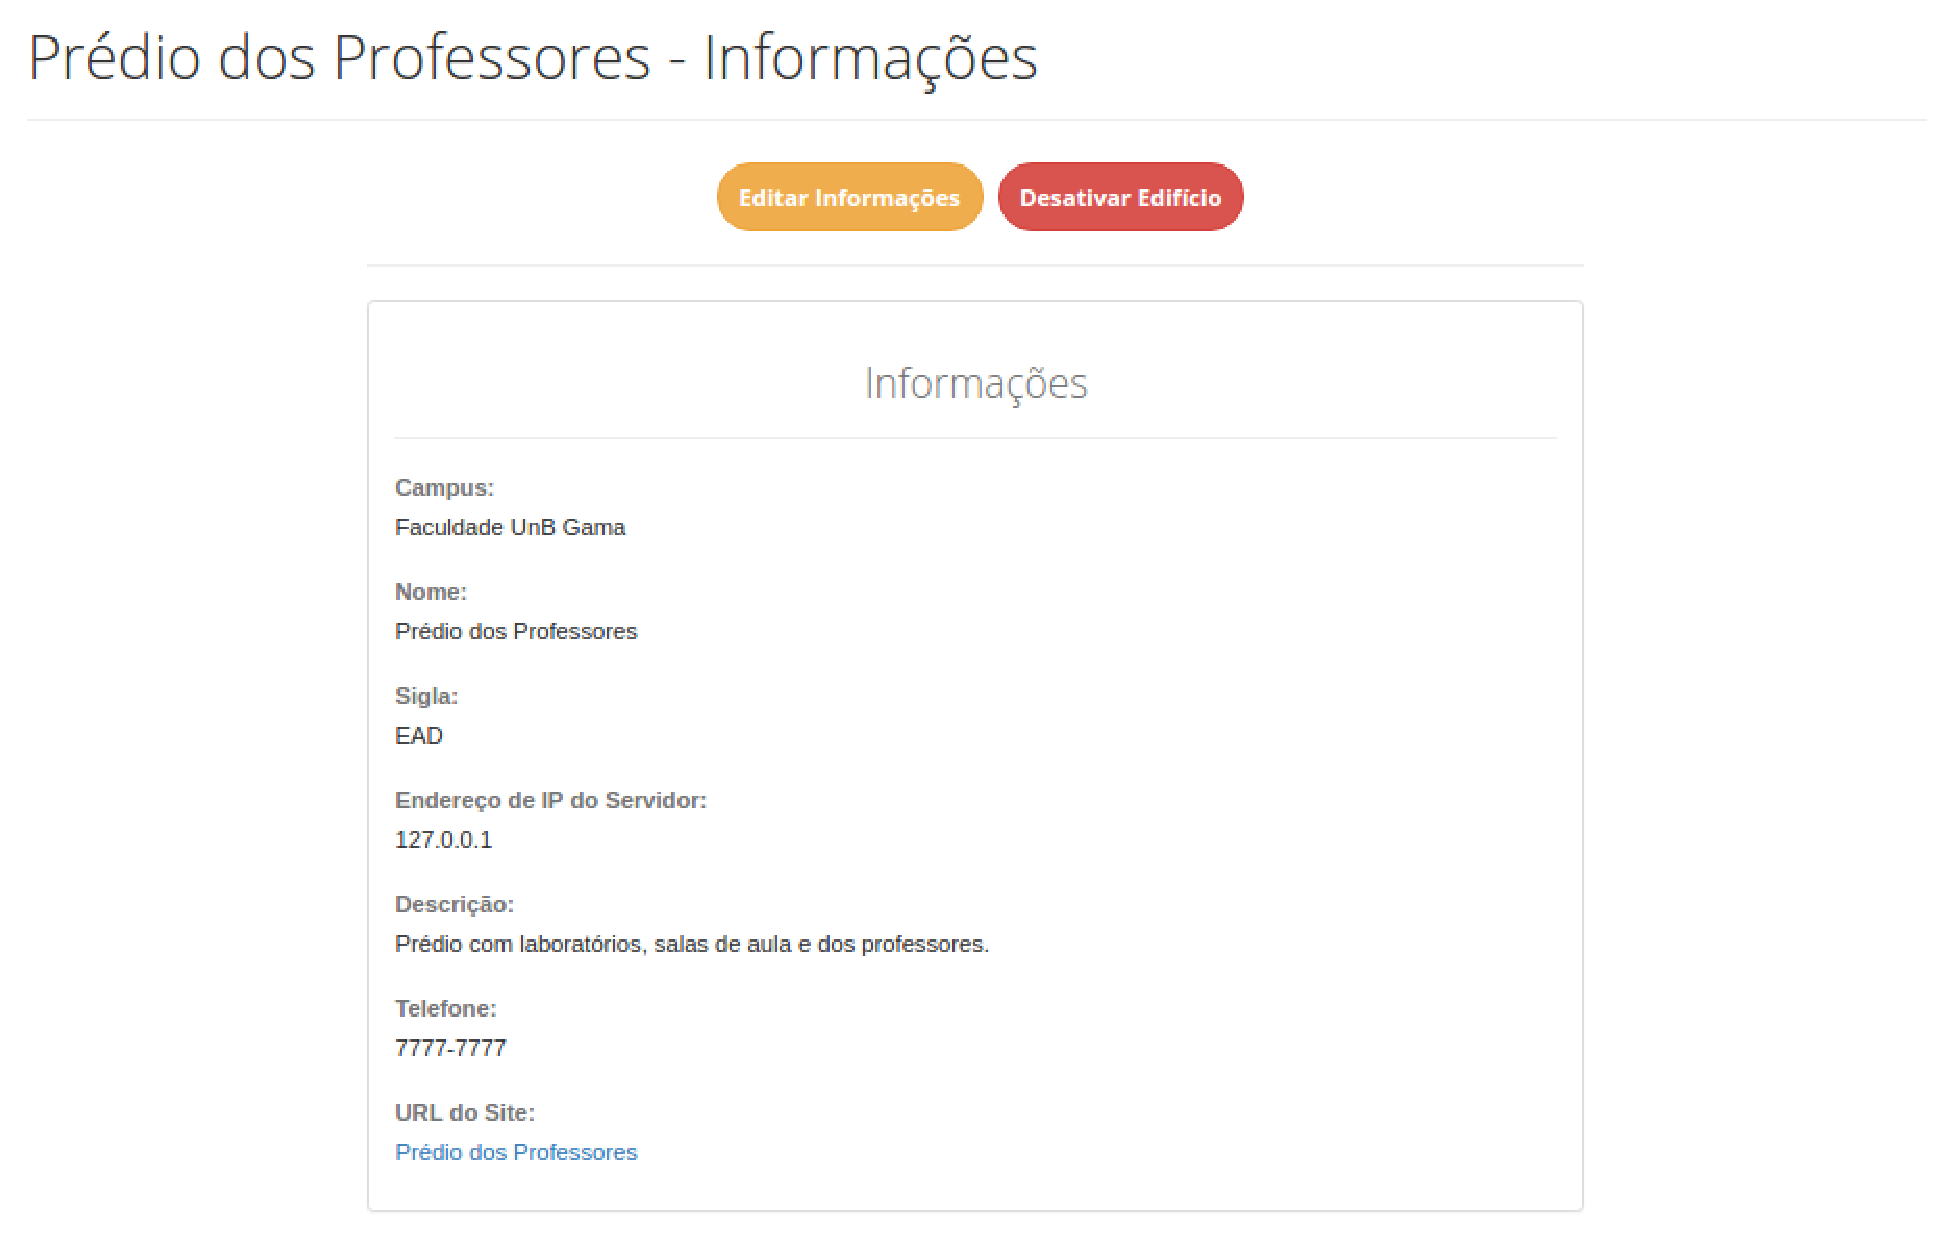
\includegraphics[keepaspectratio=true,scale=0.55]{figuras/img12.eps}
    \caption{Informações de um edifício.}
    \label{img12}
\end{figure}

\begin{figure}[!htpb]
    \centering
    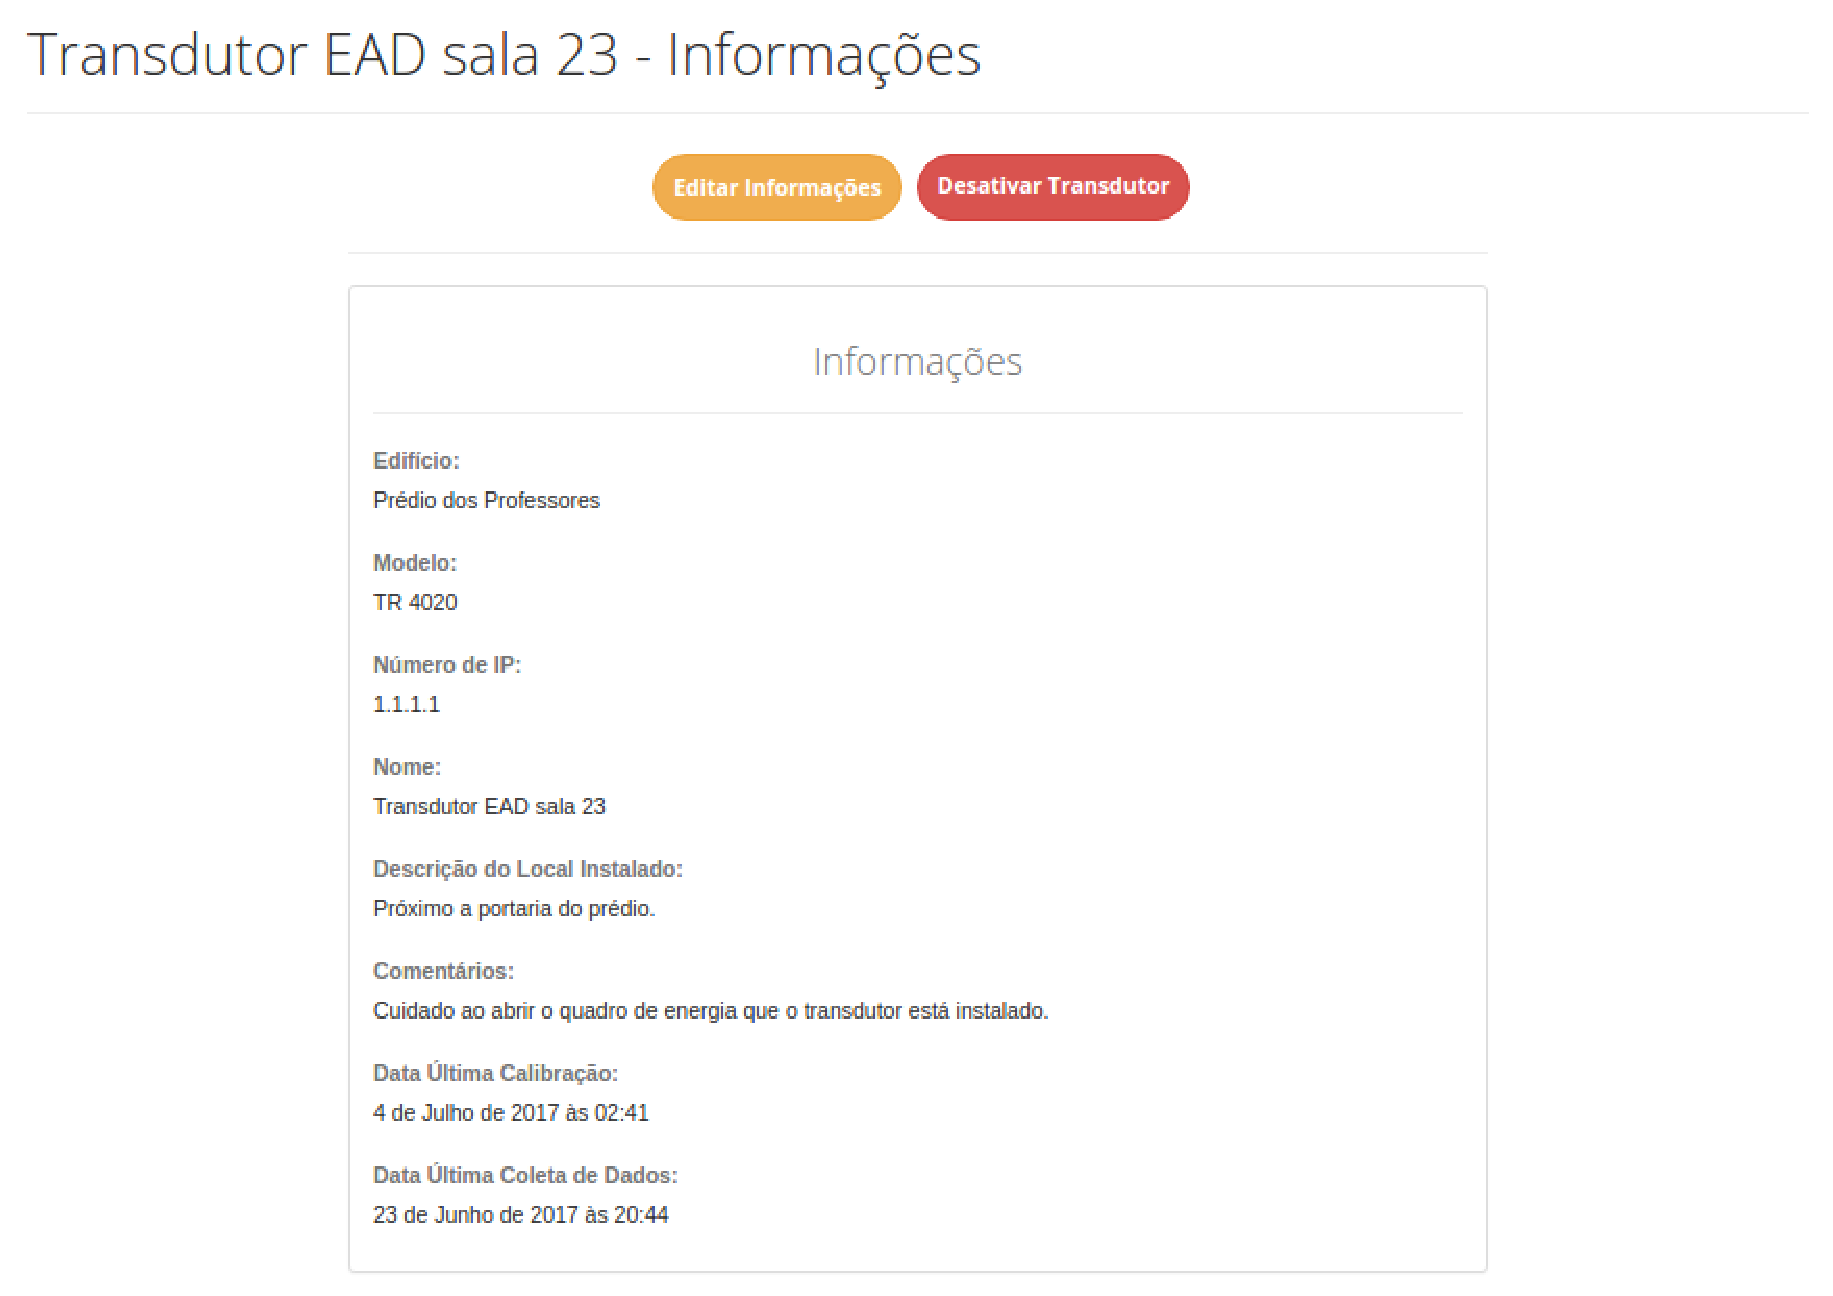
\includegraphics[keepaspectratio=true,scale=0.6]{figuras/img13.eps}
    \caption{Informações de um transdutor.}
    \label{img13}
\end{figure}

\begin{figure}[!htpb]
    \centering
    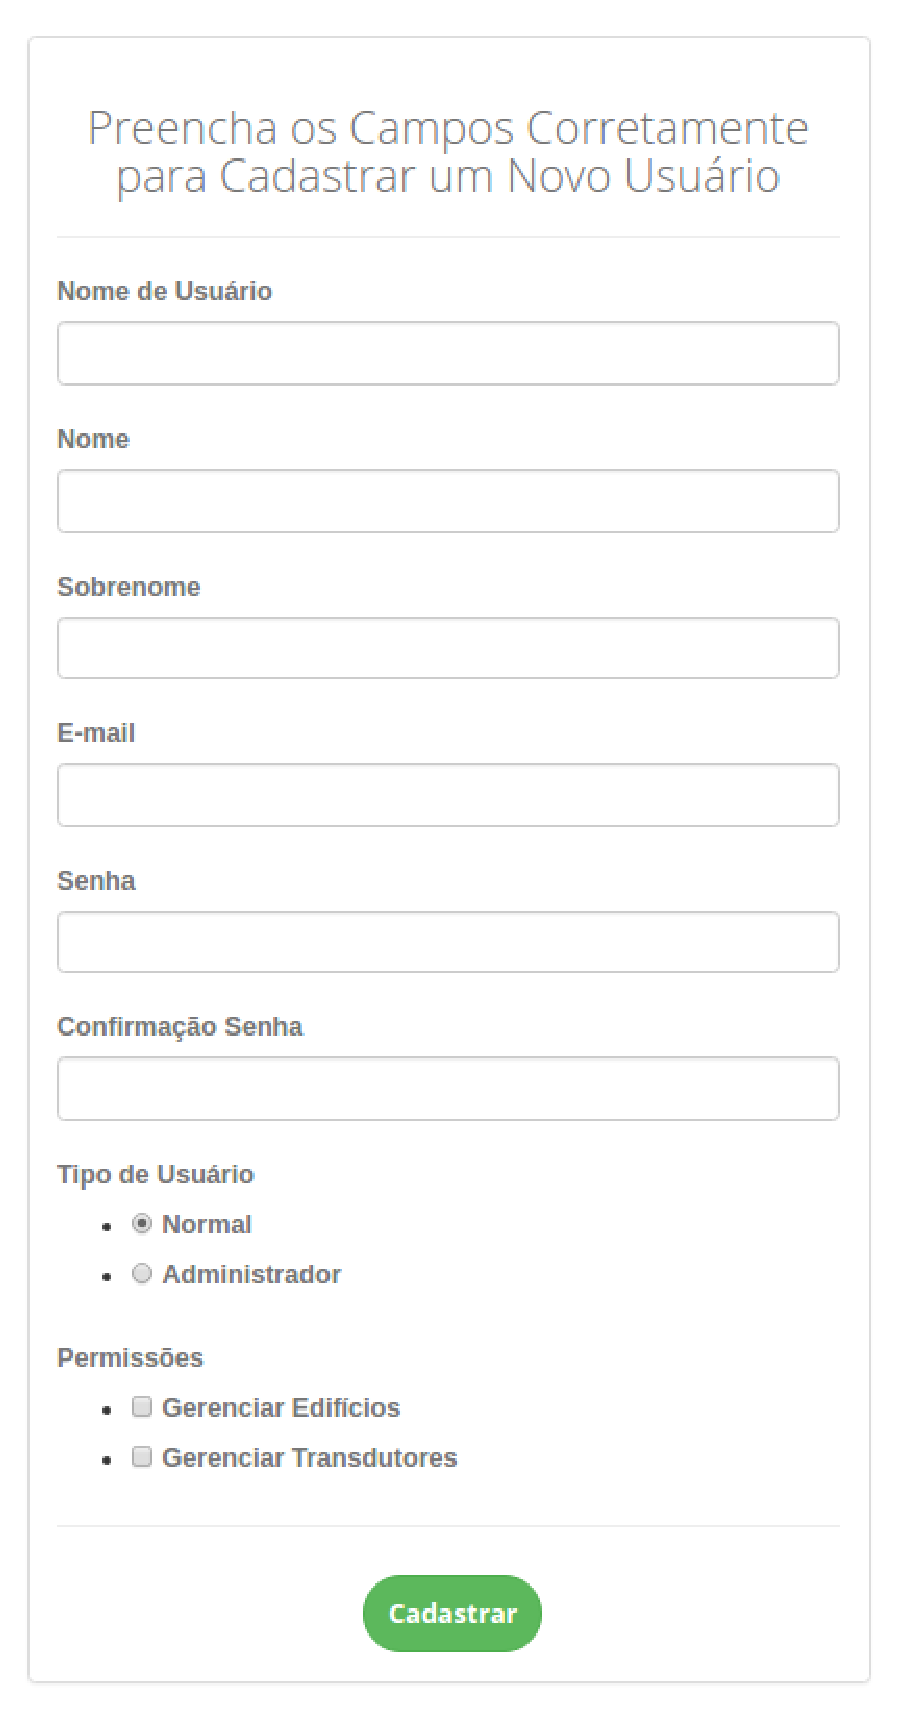
\includegraphics[keepaspectratio=true,scale=0.8]{figuras/img3.eps}
    \caption{Formulário para cadastro de um usuário.}
    \label{img3}
\end{figure}

\begin{figure}[!htpb]
    \centering
    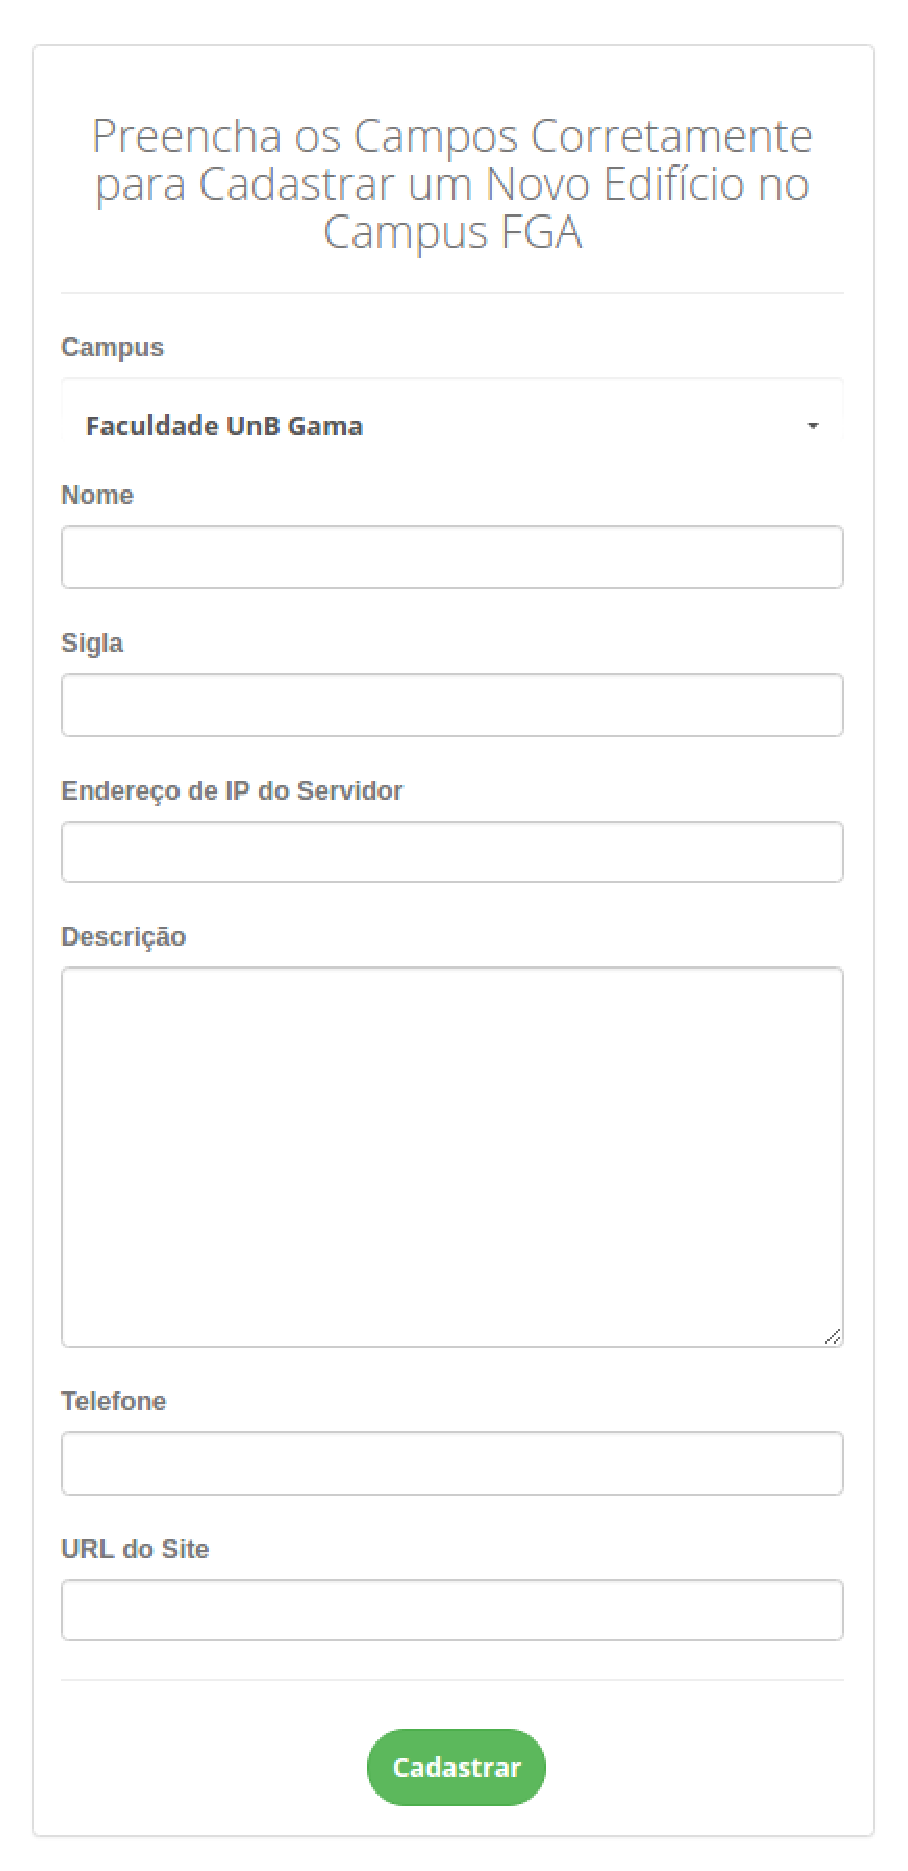
\includegraphics[keepaspectratio=true,scale=0.65]{figuras/img10.eps}
    \caption{Formulário para cadastro de um edifício.}
    \label{img10}
\end{figure}

\begin{figure}[!htpb]
    \centering
    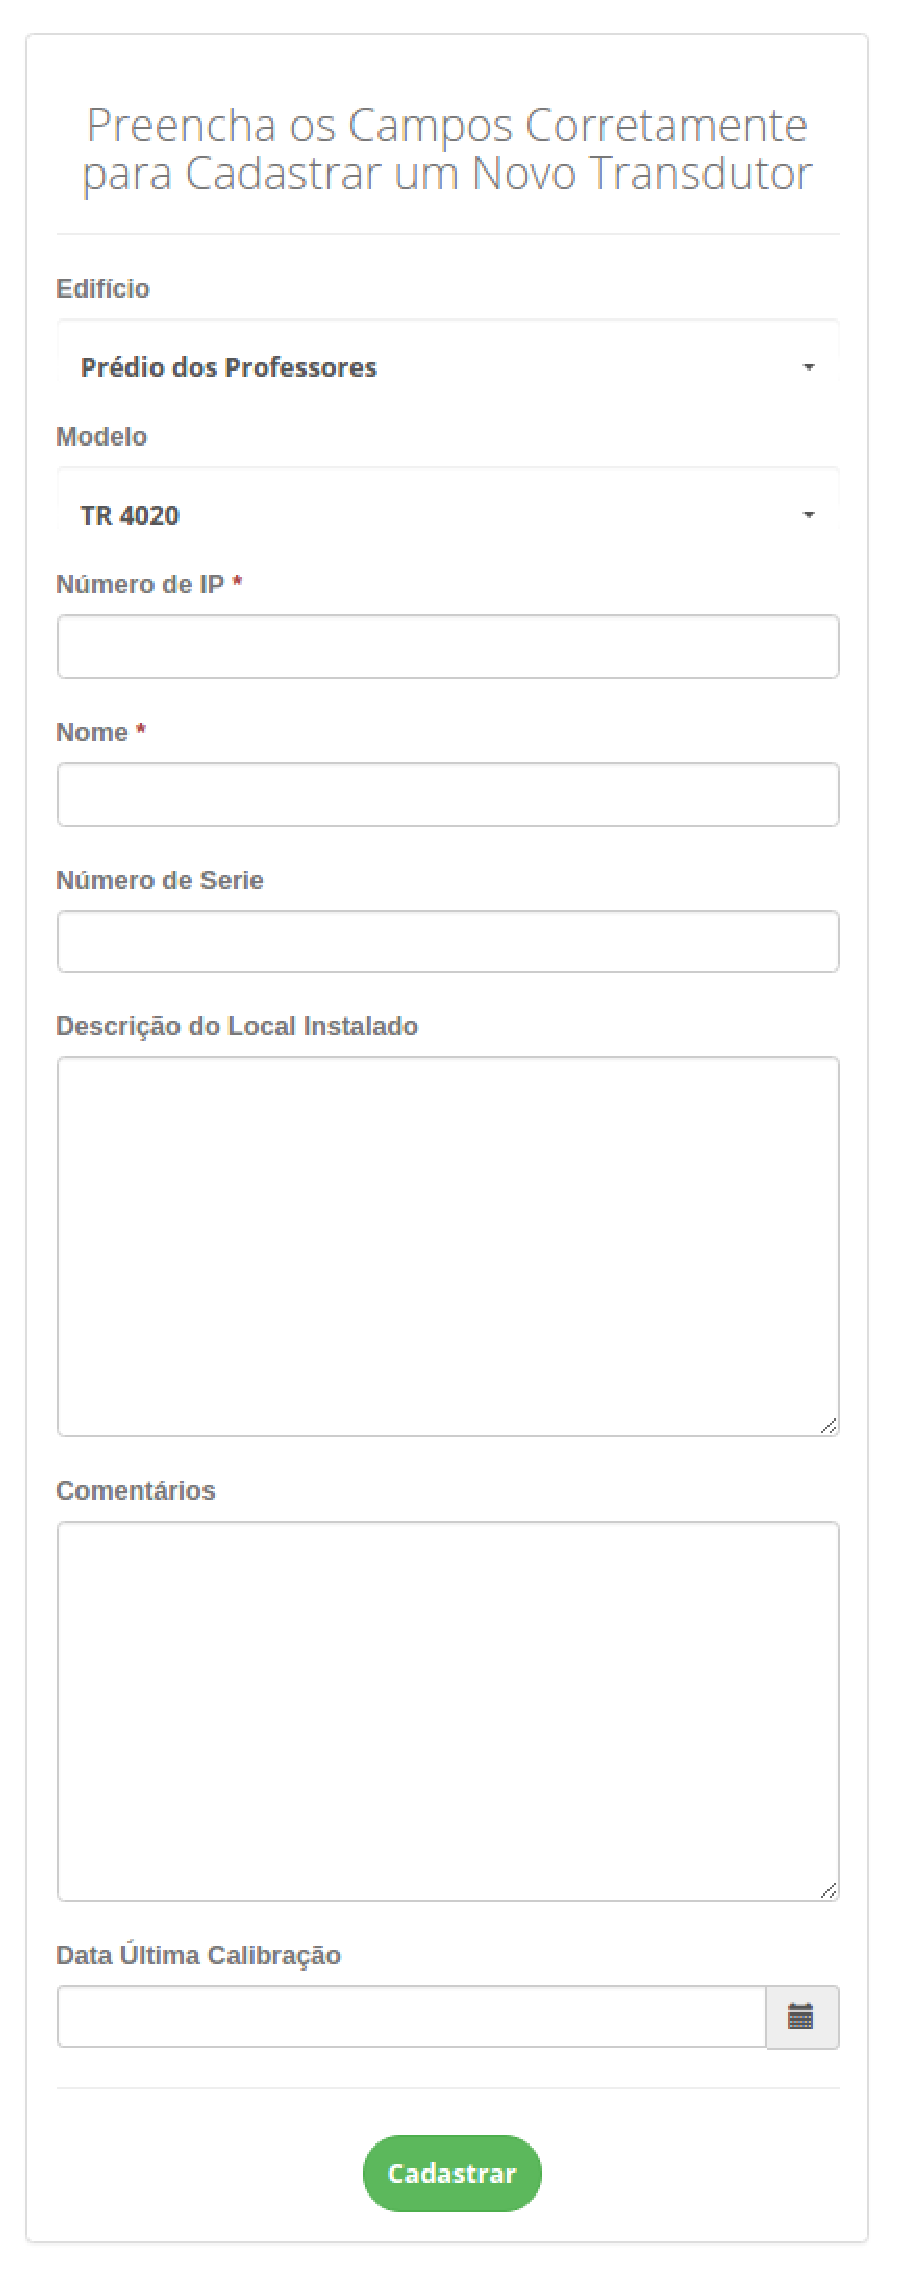
\includegraphics[keepaspectratio=true,scale=0.65]{figuras/img14.eps}
    \caption{Formulário para cadastro de um transdutor.}
    \label{img14}
\end{figure}

\end{anexosenv}